\documentclass[a4paper,envcountsame,runningheads]{llncs}
\pdfmapfile{+cm-super-t1.map}
\usepackage[T1]{fontenc}
\usepackage[utf8]{inputenc}
\usepackage{amsmath,amssymb,booktabs,array,graphicx,tikz,placeins}
\usepackage[ruled,linesnumbered]{algorithm2e}
\usetikzlibrary{arrows.meta,positioning}
\usepackage[hidelinks,hypertexnames=false]{hyperref}
\hypersetup{pdftitle={LULA I: Rollback-Resilient Hash-Based Signatures with Cache-Accelerated Signing},pdfauthor={Luis Ángel Gonzalez},pdfsubject={LULA research family of hash-based signature schemes, Ring0 Labs, published by Lugel Labs},pdfkeywords={LULA, LULA I, hash-based signatures, rollback, cache}}
\usepackage[capitalise,noabbrev]{cleveref}
\pagestyle{plain}
\renewcommand{\figurename}{Figure}
\setlength{\emergencystretch}{2em}
\newcolumntype{P}[1]{>{\raggedright\arraybackslash}p{#1}}
\newcommand{\Hh}{\mathsf{SHA256}}
\newcommand{\Tr}{\mathsf{Trunc}_{16}}
\newcommand{\KG}{\mathsf{KeyGen}}
\newcommand{\Sign}{\mathsf{Sign}}
\newcommand{\Vf}{\mathsf{Verify}}
\newcommand{\CP}{\mathsf{CachePrepare}}
\newcommand{\AD}{\mathsf{ADRS}}
\newcommand{\Th}{\mathsf{Th}}
\newcommand{\BE}{\mathsf{BE}_{4}}
\newcommand{\bits}{\mathsf{bits}}
\newcommand{\Chain}{\mathsf{Chain}}
\newcommand{\Root}{\mathsf{Root}}
\newcommand{\Auth}{\mathsf{Auth}}
\newcommand{\Ctr}{\mathsf{FirstCounter}}
\newcommand{\Adv}{\mathsf{Adv}}
\newcommand{\eps}{\varepsilon}
\SetKw{Return}{return}
\SetKwInput{Input}{Input}
\SetKwInput{Output}{Output}
\begin{document}
\raggedbottom
\title{LULA I: Rollback-Resilient Hash-Based Signatures with Cache-Accelerated Signing}
\titlerunning{LULA I: Cache-Accelerated Hash-Based Signatures}
\author{Luis \'Angel Gonzalez}
\authorrunning{L.\,\'A. Gonzalez}
\institute{Ring0 Labs\\Published by Lugel Labs}
\maketitle
\thispagestyle{plain}
\begin{abstract}
LULA is Ring0 Labs' research family of hash-based signature schemes. This first paper presents LULA I, a deterministic signer accelerated by reusable caches. For successfully generated keys and honest prepared, restored or absent caches, we prove reference-signer agreement on termination and returned signature bytes. An atomic rollback simulation transfers an applicable reference bound without signing-query loss; the complete reference-signer bound remains open. Signatures are 5,720 bytes; cache payload is approximately 72 MiB. Six gated blocks on one host gave pooled prepared-signing medians of 3.56--3.64 ms across three message lengths. Separate historical and first-campaign prepared-signing median bands were 5.6--9.5 and 3.9--4.6 ms. Three individual first signatures after cache loss took 330.049--337.563 s. These observations establish no common-security ranking. The SHRINCS counter-reuse discussion is a model argument; no forgery attack against a real implementation was run.
\keywords{Hash-based signatures \and Rollback \and Caching \and WOTS+C \and FORS+C}
\end{abstract}

\section{Introduction}\label{sec:introduction}
LULA is Ring0 Labs' research family of hash-based signature schemes. This first paper presents LULA I and studies how honest cache restoration affects the signing function and its computation cost.

An adaptive adversary may obtain signatures from several executions of the same signer, each resumed from an older snapshot. The adversary retains the union of signatures published across these executions. A resource that appears unused in every restored execution may nevertheless have been exposed in another branch. Consequently, protecting a local consumption counter does not by itself protect a hash-based signing key against restoration.

The question studied here is whether mutable state can accelerate a hash-based signer without controlling which authorization resources it consumes. LULA I answers a restricted version constructively: its cache stores computations for a single deterministic reference signing function. Whenever signing terminates, the same message and key produce the same signature after an honest cache restoration, after cache deletion, or with caching disabled. Under these honest cache conditions, the cache changes computation time while preserving the signature bytes whenever signing terminates. Any unforgeability claim after restoration remains conditional on an applicable bound for the common reference signer.

The author-selected use objective is $2^{40}$ signing queries across all branches, conditional on a still-unestablished full reference-signer bound. The classical FORS+C component model and its unresolved assumptions are stated once in \Cref{sec:operating}.

A large upper Merkle tree can be computed once and retained, while signing recomputes only smaller lower trees. Counters used to search for acceptable WOTS+C digests can also be prepared for message-independent child roots. Counter selection must be canonical: two counters for the same root can select different digests. Caching a counter without specifying its recomputation rule can therefore introduce the multiple-exposure problem that caching was intended to avoid.

Stateless hash-based signatures, their caches, and counter-based compression are established techniques. SPHINCS+ supplies the underlying FORS/hypertree architecture~\cite{sphincs}; SPHINCS+C supplies compressed component designs~\cite{sphincsc}; Gravity-SPHINCS already uses secret-key caching~\cite{gravity}. LULA I is an implementation and security-boundary case study of this stateless architecture. We make no claim to have introduced stateless signing or caching as cryptographic principles. Its unforgeability remains conditional on the reference-signer premise in \Cref{sec:security,thm:transfer}.

Cache loss changes computation time even when signature bytes are preserved. Our parameter set has a height-21 cached top tree. Its removal requires billions of online compressions. Historical sessions, the first campaign, and the gated follow-up measured this cost separately (\Cref{sec:experiments,sec:benchcomparison,sec:stability}). Their elapsed-time differences are not a controlled optimization comparison. Output invariance and recovery cost are distinct properties of the mechanism.

\subsection{Contributions and scope}\label{sec:scope}

\begin{enumerate}
\item[\textbf{C1.}] We specify one parameter set, its complete wire format, and its signature, cache, and work accounting (\Cref{sec:construction,sec:cache,sec:cost}).
\item[\textbf{C2.}] We prove deterministic cache transparency, including termination equivalence, for successfully generated keys and honest cache states (\Cref{lem:transparent}).
\item[\textbf{C3.}] We give a rollback-game simulation conditional on the common reference signer's security, and a counterexample to a general converse from frozen-state security (\Cref{sec:rollback}).
\item[\textbf{C4.}] We analyze canonical counters and reproduce bounded negative controls for noncanonical counters and restored randomness (\Cref{sec:security,sec:experiments}).
\item[\textbf{C5.}] We measure cache lifecycle costs and compare implementations, retaining separate execution contexts and the limits of the first campaign and gated follow-up (\Cref{sec:experiments,sec:benchcomparison,sec:stability}).
\end{enumerate}

The security result is a transfer theorem: rollback access preserves any applicable security bound for the common reference signing algorithm. It does not derive that reference bound from the underlying hash construction. The proof concerns honest snapshot restoration and atomic completed-call observations; edited cache contents, interrupted execution and leakage require different interfaces.

The paper proceeds in this order. \Cref{sec:introduction} introduces the question and includes the contributions and scope in \Cref{sec:scope}. \Cref{sec:related,sec:notation} cover related work and notation; \Cref{sec:game,sec:construction,sec:correctness} give the threat model, construction and correctness. \Cref{sec:security,sec:rollback} present the security analysis and rollback transfer. \Cref{sec:cache,sec:cost,sec:implementation} describe caching, signing-query reference points, wire format and computation, and implementation. \Cref{sec:experiments,sec:stability,sec:benchcomparison} report historical measurements and replay, the gated follow-up, and the first-campaign comparison. \Cref{sec:limits,sec:conclusion} state the operational boundaries and conclusion. \Cref{app:search,app:falsifiers} give counter-search costs and the claim-to-falsifier map.

\section{Related work}\label{sec:related}
\paragraph{Stateful and stateless authorization.}
XMSS authenticates one-time keys with Merkle paths and requires that an index not be reused~\cite[Sections~4.1 and 4.1.9]{xmss}. SPHINCS+ uses a few-time component selected by a message digest and certifies it through a hypertree~\cite{sphincs}. SLH-DSA standardizes this architecture with specified hash functions and parameters~\cite{fips205}. LULA I follows the stateless architecture, rather than attempting to make a consumption index survive restoration. Unforgeability under restoration still depends on the reference-signer premise in \Cref{sec:security,thm:transfer}.

\paragraph{Compressed components and variable layers.}
SPHINCS+C searches for digest subsets that permit shorter WOTS and FORS evidence~\cite{sphincsc}. A fixed digit sum replaces a conventional checksum in the WOTS+C component considered here. Kudinov and Nick analyze alternative component choices~\cite[Sections 5 and 13]{kn}. Qin, Sun, and Zheng consider varying heights and chain lengths across layers~\cite{variable}. LULA I uses different heights and widths at different layers; these choices define the concrete signing function whose cache behavior we study.

\paragraph{Caching and reset attacks.}
Gravity-SPHINCS demonstrates that caching can change signing cost and the parameter tradeoff~\cite{gravity}. Ristenpart and Yilek analyze virtual-machine reset vulnerabilities and hedging against randomness failures~\cite{reset}. Our deterministic signer consumes no online random-generator state. It therefore avoids dependence on a restored generator, conditional on the security of its message-dependent derivation. This does not establish that determinism alone implies security.

\paragraph{Limited-use parameter sets.}
NIST SP 800-230's initial public draft proposes additional SLH-DSA parameter sets with a $2^{24}$ lifetime signature limit and permits hypertree caching~\cite[Table~1 and Section~3]{sp800230}. Its 3,856-byte SHA2-128-24 signatures illustrate why query limits must accompany size comparisons; this draft set was not measured here. Fluhrer and Dang analyze FORS coverage using an occupancy model~\cite[Section~5]{fluhrer}; \Cref{sec:operating} states the additional modeling assumptions used for LULA I.

\paragraph{Positioning.}
The recovered third-party Go implementation selects the smallest valid WOTS+C counter, including in its parallel search~\cite{hashsiggo}. The supported contribution is the exact integration and audit of canonical counter caching, together with measured lifecycle costs. Establishing novelty beyond prior implementations would require a broader implementation comparison. This paper claims neither a new hardness assumption nor a new general security property of stateless signatures.

\section{Preliminaries and notation}\label{sec:notation}
All hash nodes are $n=16$ bytes. $\Hh$ produces 32 bytes; $\Tr$ selects its first 16 bytes. Concatenation is denoted by $\|$. All integer fields use big-endian byte order. $\BE(c)$ encodes a 32-bit unsigned integer. $\bits(D,s,r)$ reads $r$ bits starting at zero-based bit offset $s$, most-significant bit first. Messages are finite byte strings $M$ with length $L$.

For a binary Merkle tree of height $h$, a path contains $h$ sibling nodes, from the leaf upward. At each level the index parity determines the left/right order. The address includes the height and parent index. A subtree is represented in level-major order: leaves first, then each successive level, ending at the root.

The hypertree has $d$ layers numbered $j=0,\ldots,d-1$ from bottom to top. Layer $j$ has height $h_j$, width $w_j=2^{b_j}$, and $\ell_j=128/b_j$ WOTS chains. The evaluated set has no forced-zero WOTS digits. Its required digit sum is $S_j=\ell_j(w_j-1)/2$. Define $h=\sum_j h_j$ and $s_j=\sum_{i<j}h_i$. For an $h$-bit index $I$, the leaf and tree indices are
\begin{equation}\label{eq:route}
 q_j=(I\mathbin{\gg}s_j)\bmod 2^{h_j},\qquad
 t_j=I\mathbin{\gg}(s_j+h_j).
\end{equation}
The FORS+C digest addresses $k$ trees of height $a$ but forces the last index to zero. Only $k'=k-1$ trees are instantiated and transmitted. This omission is part of the compressed construction; no secret from an omitted tree is serialized.

\section{Threat model and security definitions}\label{sec:game}
\subsection{Atomic chosen-message rollback game}
Let $\Pi=(\KG,\Sign,\Vf)$ be a signature scheme whose key-generation algorithm $\KG$ returns a public key $pk$, a secret key $sk$, and initial mutable state $\mu_0$. A challenger gives $pk$ to an adversary $\mathcal A$ and maintains a current state, a handle-indexed snapshot store, and a permanent message set $\mathcal Q$. The initial snapshot has handle 0; subsequent snapshots receive sequential integer labels that disclose no state contents. The following commands are allowed:
\begin{itemize}
\item $\mathsf{Sign}(M)$ returns $\sigma$ and updates the current state atomically; it adds $M$ to $\mathcal Q$.
\item $\mathsf{Snapshot}()$ stores the complete current restorable state and returns an opaque handle.
\item $\mathsf{Restore}(u)$ restores a previously stored snapshot. It does not remove messages from $\mathcal Q$ or erase the adversary's observations.
\end{itemize}
The adversary may restore the initial snapshot or snapshots between any two completed signing calls, branch repeatedly, and choose its next message adaptively. State contents remain secret. Restoration installs an honest earlier state of the same key and parameter set; arbitrary edited bytes are not a restoration operation in this game.

At most $Q$ signing queries are counted across all branches. The adversary also has computational budget $T$ and, in a random-oracle formulation, at most $q_H$ adversarial hash-oracle queries. The time budget counts local adversary and simulator computation; the honest signing oracle's internal work is accounted for separately in \Cref{sec:cost}. Snapshot and restoration commands are finite and bounded by the adversary's total resources, but no fixed security-critical restoration limit is imposed. A fresh-message forgery wins when
\begin{equation}\label{eq:win}
 \Vf(pk,M^*,\sigma^*)=1\quad\text{and}\quad M^*\notin\mathcal Q.
\end{equation}
Define $\Adv^{\mathrm{euf\text{-}cma\text{-}rb}}_{\Pi}(\mathcal A)$ as the probability of this event over key generation, adversarial coins, and any explicitly modeled hash or signing randomness. The definition is parameterized by $(Q,T,q_H)$; fixing $Q$ alone does not specify a concrete security level.

Ordinary existential unforgeability under chosen-message attacks (EUF-CMA) removes snapshot and restoration commands. It uses the same permanent freshness set. We study existential unforgeability, not strong unforgeability: another signature on a queried message is not a winning forgery.

\subsection{Randomness and excluded observations}
In a restored-randomness model, generator state is part of the snapshot. In a fresh-entropy model, new independent coins remain available after restoration. LULA I's implemented signer is deterministic given $(sk,M)$ and does not call either generator, so both models induce the same outputs. Key generation still requires securely sampled secret material; benchmark seeds are deterministic fixtures, not production entropy sources.

The game omits elapsed times, crash behavior, partial signatures, and access to the cache bytes. It therefore proves no timing noninterference or leakage guarantee. Mid-call restoration is excluded by atomicity. A nonterminating signing request prevents that experiment from reaching a winning completion. A real implementation that publishes partial work, resumes corrupted execution frames, or reveals timing information needs a stronger model.

\section{LULA I construction}\label{sec:construction}
\subsection{Parameters and key material}
\Cref{tab:params} fixes one parameter set throughout this paper. Its digest uses $ka+h=203$ of the 256 output bits, including nine forced-zero bits. The public key is $PK.seed\|PK.root$ (32 bytes). The stored master seed is $SK.seed\|SK.prf\|PK.seed$ (48 bytes); each component is 16 bytes. The public root is also retained by the signer. Expanded context and allocations are additional memory, not additional transmitted key fields.

\begin{table}[t]
\caption{The single evaluated LULA I parameter set. The last column identifies prepared layers; it is not an authorization counter.}\label{tab:params}
\centering\small
\begin{tabular}{lrrrrrl}\toprule
Component & $h_j$ & $b_j$ & $w_j$ & $\ell_j$ & $S_j$ & Cache\\\midrule
Layers 0--3, each &5&4&16&32&240&No\\
Layer 4 &21&8&256&16&2040&Yes\\\bottomrule
\end{tabular}

\smallskip
\begin{tabular}{lr@{\quad}lr}\toprule
Node bytes $n$&16&Total height $h$&41\\
FORS digest trees $k$&18&FORS height $a$&9\\
Transmitted trees $k'$&17&Hypertree layers $d$&5\\\bottomrule
\end{tabular}
\end{table}

\subsection{Addresses and hashes}\label{sec:hash}
An address is exactly 22 bytes:
\[
 \AD=\mathsf{layer}_1\|\mathsf{tree}_8\|\mathsf{type}_1
       \|\mathsf{keypair}_4\|\mathsf{word2}_4\|\mathsf{word3}_4.
\]
Subscripts give field sizes in bytes. Types 0--7 denote WOTS chain, WOTS public-key compression, hypertree node, FORS node, FORS-root compression, WOTS-secret derivation, FORS-secret derivation, and WOTS+C message digest, respectively. Word 2 is a chain index or tree height; word 3 is a chain position or node index. Unused fields are zero. These types separate the implemented domains; they do not imply that arbitrary uses of SHA-256 satisfy all required cryptographic assumptions.

For byte string $X$, the implemented tweakable function is
\begin{equation}\label{eq:th}
 \Th(A,X)=\Tr\bigl(\Hh(PK.seed\|0^{48\,\mathrm{bytes}}\|A\|X)\bigr).
\end{equation}
The leaf function is $F(A,x)=\Th(A,x)$ and the binary node function is $H(A,x,y)=\Th(A,x\|y)$. Secret derivation uses $\mathsf{PRF}(A)=\Th(A,SK.seed)$. SHA-256's compression state after the first 64-byte prefix is prepared once per context. No nonstandard compression padding is introduced.

The message functions are
\begin{align}\label{eq:message}
 R(M)&=\Tr\bigl(\Hh(SK.prf\|PK.seed\|M)\bigr),\nonumber\\
 U(M)&=\Hh(R(M)\|PK.seed\|PK.root\|M),\\
 D_c(M)&=\Hh(U(M)\|\BE(c)\|PK.seed).\nonumber
\end{align}
The signer selects the smallest $c\in\{0,\ldots,2^{32}-1\}$ for which $\bits(D_c,153,9)=0$. The first 153 bits select 17 FORS indices; bits 162--202 select $I$. Verification recomputes these values using transmitted $R$ and $c$, rather than checking that $R$ was secretly derived. Consequently, an unforgeability argument must cover adversarial choices of both fields.

These functions differ from standardized SLH-DSA's HMAC-based message randomizer, message expansion, and external context interface~\cite[Sections~10.2, 10.3, and 11.2]{fips205}. LULA I is not SLH-DSA conformant. Its raw-message interface provides no standardized application-context or prehash wrapper.

\subsection{WOTS+C keys}
For address $(j,t,q)$ and a 16-byte value $V$, let
\[
 E_c(V)=\Th(\AD(j,t,7,q,0,0),V\|\BE(c)).
\]
Read $E_c(V)$ as $\ell_j$ base-$w_j$ digits $e_0,\ldots,e_{\ell_j-1}$. A counter is accepted when $\sum_i e_i=S_j$. $\Ctr(j,t,q,V)$ returns the smallest accepted counter. The secret chain start is
\[
 x_i=\mathsf{PRF}(\AD(j,t,5,q,i,0)).
\]
To advance from position $u$ by $v$ steps, apply $F(\AD(j,t,0,q,i,p),\cdot)$ successively for $p=u,\ldots,u+v-1$. The public key is the type-1 compression of all endpoints at position $w_j-1$. A signature on $V$ contains $c$ and the $\ell_j$ chain values at positions $e_i$. Verification completes each chain and compresses the endpoints.

Layer-tree leaves are these WOTS public keys. A type-2 address identifies each Merkle node by $(j,t,\text{height},\text{index})$. The child value signed at layer 0 is the FORS public key associated with $(t_0,q_0)$. For layer $j>0$, it is the root of subtree $(j-1,\,t_j2^{h_j}+q_j)$. Both values are fixed by the key and address, independently of the message that routes through them.

\subsection{FORS+C component}
For tree $r\in\{0,\ldots,16\}$ and leaf $i<512$, define the global index $g=512r+i$. The secret is the type-6 PRF at $(0,t_0,q_0,g)$; its leaf image is the type-3 hash at height zero and index $g$. At height $v$, the address index is $r2^{a-v}+i_v$, where $i_v$ is the local index at that level. A FORS signature reveals one selected secret and its nine siblings per tree. A type-4 compression of the 17 reconstructed roots gives $V_0$.

The implementation instantiates only the 17 real trees; no implicit secret is transmitted for the omitted tree. Both signing and verification enforce the zero condition on the eighteenth index.

\subsection{Key generation and cache preparation}
\Cref{alg:kg,alg:prepare} present key generation and cache preparation separately; the executable key-generation routine also prepares the configured caches. The mathematical key-generation interface requires a securely sampled seed, whereas the executable routine receives its seed from the caller. LULA I prepares only the top-layer cache, containing one height-21 subtree and one canonical counter for each of its $2^{21}$ leaves. Preparing a counter requires the corresponding height-5 child root.

\begin{algorithm}[t]
\caption{LULA I KeyGen}\label{alg:kg}
\Input{Parameters in \Cref{tab:params}; securely sampled 48-byte seed $s$}
\Output{$(pk,sk,C)$}
Split $s$ into $(SK.seed,SK.prf,PK.seed)$\;
Initialize the seed-derived hash context $\mathsf{ctx}$ from $(SK.seed,SK.prf,PK.seed)$, including the SHA-256 prefix state\;
$C\leftarrow\CP(\mathsf{ctx})$ using \Cref{alg:prepare}\;
$PK.root\leftarrow C.\mathsf{topTree}.\mathsf{root}$\;
$pk\leftarrow PK.seed\|PK.root$\;
\Return{$(pk,(s,PK.root),C)$}\;
\end{algorithm}

\begin{algorithm}[t]
\caption{LULA I CachePrepare}\label{alg:prepare}
\Input{Seed-derived hash context $\mathsf{ctx}$ and fixed parameters}
\Output{Top-tree nodes and canonical counters}
\For{$q=0,\ldots,2^{21}-1$}{
 $y_q\leftarrow\mathsf{WotsPK}(4,0,q)$\;
 $V_q\leftarrow\Root(\mathsf{Subtree}(3,q))$\;
 $c_q\leftarrow\Ctr(4,0,q,V_q)$\;
}
$T\leftarrow\mathsf{MerkleBuild}(4,0,y_0,\ldots,y_{2^{21}-1})$\;
\Return{$C=(T,(c_q)_{q<2^{21}})$}\;
\end{algorithm}

\subsection{Signing and public verification}
\Cref{alg:sign,alg:verify} specify the transmitted object, including every counter. Neither algorithm consults a consumption index. An honest cache entry changes which computations are repeated; it does not change their outputs. Unforgeability under restoration still requires the reference-signer premise in \Cref{sec:security,thm:transfer}.

\begin{algorithm}[t]
\caption{LULA I Sign}\label{alg:sign}
\Input{$(sk,PK.root,C,M)$}
\Output{Serialized signature $\sigma$}
Compute $R,U$ from \Cref{eq:message}\;
$c_F\leftarrow$ smallest counter with $\bits(D_{c_F},153,9)=0$\;
Extract $i_0,\ldots,i_{16}$ and $I$ from $D_{c_F}$\;
Derive $(t_0,q_0)$ from \Cref{eq:route}\;
$(\sigma_F,V)\leftarrow\mathsf{ForsSign}(t_0,q_0,(i_r)_r)$\;
$\sigma\leftarrow R\|\BE(c_F)\|\sigma_F$\;
Let $x_i^{(j)}$ denote the secret chain starts at leaf $(j,t_j,q_j)$, as defined in the WOTS+C section\;
\For{$j=0,\ldots,4$}{
 Derive $(t_j,q_j)$ from \Cref{eq:route}\;
 Obtain $(c,T)$ by \Cref{alg:restore}\;
 $e\leftarrow$ digits of $E_c(V)$\;
 $W\leftarrow(\Chain(x_i^{(j)},0,e_i))_{i<\ell_j}$\;
 $\sigma\leftarrow\sigma\|\BE(c)\|W\|\Auth(T,q_j)$\;
 $V\leftarrow\Root(T)$\;
}
\Return{$\sigma$}\;
\end{algorithm}

\begin{algorithm}[t]
\caption{LULA I Verify}\label{alg:verify}
\Input{$(pk,M,\sigma)$}
\Output{Boolean}
Reject unless $|pk|=32$ and $|\sigma|=5720$\;
Parse fields in the order of \Cref{tab:wire}\;
Recompute $U,D_{c_F}$ from transmitted $R,c_F$ and $(pk,M)$\;
Reject unless $\bits(D_{c_F},153,9)=0$\;
Extract FORS indices and $I$; derive $(t_0,q_0)$\;
$V\leftarrow\mathsf{ForsPKFromSig}(t_0,q_0,(i_r)_r,\sigma_F)$\;
\For{$j=0,\ldots,4$}{
 Derive $(t_j,q_j)$; read the layer counter $c_j$\;
 $e\leftarrow$ digits of $E_{c_j}(V)$\;
 Reject unless $\sum_i e_i=S_j$\;
 Reconstruct WOTS public key by completing each chain\;
 $V\leftarrow\mathsf{RootFromPath}(j,t_j,q_j,\mathsf{WotsPK},\mathsf{path}_j)$\;
}
\Return{$V=PK.root$}\;
\end{algorithm}

The executable verifier receives the two fixed-size public-key nodes as typed arguments. Its byte-signature parser rejects nonexact signature length before reading fields. The public-key byte-length rejection in \Cref{alg:verify} belongs to the mathematical serialization interface, rather than to a separately implemented raw-public-key parser.

\begin{algorithm}[t]
\caption{LULA I CacheRestore: cache lookup and cache-miss recomputation}\label{alg:restore}
\Input{Layer $j$, route $(t,q)$, current child value $V$, honest cache $C$}
\Output{Counter $c$ and subtree $T$}
\eIf{$j=4$ and the complete top-layer cache is present}{
 $T\leftarrow C.\mathsf{topTree}$; $c\leftarrow C.\mathsf{counters}[q]$\;
 \If{$c$ does not satisfy the digit-sum predicate for $V$}{
 $c\leftarrow\Ctr(j,t,q,V)$\;
 }
}{
 $c\leftarrow\Ctr(j,t,q,V)$\;
 $T\leftarrow\mathsf{BuildSubtree}(j,t)$\;
}
\Return{$(c,T)$}\;
\end{algorithm}

Restoration copies an honest snapshot. The library exposes optional in-memory layer caches; it implements neither a persistent snapshot codec nor a per-entry sparse-cache protocol. \Cref{alg:restore} describes cache lookup and the miss branch; it provides no validation guarantee for arbitrary malformed cache containers.

\section{Correctness}\label{sec:correctness}
\begin{lemma}[Chain and tree reconstruction]\label{lem:correct}
For a successfully generated key and terminating counter searches, a signature produced with honest cache contents is accepted by the verifier.
\end{lemma}
\begin{proof}
Completing a chain from its signed position $e_i$ applies the remaining $w_j-1-e_i$ addressed hashes, yielding the same endpoint used in its public key. Public-key compression therefore reconstructs the corresponding leaf. Each authentication path then reconstructs its subtree root with the same addressed left/right ordering. FORS reconstruction begins with the revealed secret and reconstructs its selected leaf and root in each of the 17 trees. Its root compression equals the value signed at layer 0. Induction over the five hypertree layers gives the top-tree root fixed at key generation. The digest predicates hold by the counter searches. The serialized length equals the parser's required length by \Cref{eq:size}.\qed
\end{proof}

Counter searches are partial computations. The source increments a 32-bit integer without specifying an exhaustion error. If a search fails, overflow in a release build can wrap and revisit counters; a checked build can panic. \Cref{lem:correct} is conditional on termination. A deployable API needs explicit search-exhaustion and failure semantics.

\section{Security analysis}\label{sec:security}
\subsection{Scope of the transfer argument}
The security of the reference signer is a premise of the rollback transfer. The mechanism does not establish primitive or composition bounds for its secret derivations, message randomizer, FORS disclosure, WOTS+C substitutions or Merkle compressions. An applicable reference bound must cover the exact signing function and the public verifier, including adversarial choices of the transmitted randomizer and counters.

The transfer proof compares the public signing interfaces and does not depend on a particular hash idealization. Its signing-query and adversarial hash-query accounting excludes honest oracle-internal work, which changes with cache availability. The result concerns preservation of a reference bound under the declared restoration interface.

\subsection{Constant-sum chains and repeated certification}
For two accepted digit vectors $e,e'$ with the same sum $S_j$, componentwise domination $e'_i\ge e_i$ for all $i$ implies $e'=e$. Thus one WOTS+C exposure cannot reach a different accepted digit vector solely by advancing every chain. This antichain fact explains the target-sum predicate, but leaves digest collisions, inversions, multi-target attacks, and certification composition to the cryptographic proof.

When two distinct accepted vectors are exposed at the same address, their coordinatewise minima can have sum below $S_j$. A new target vector can then dominate those minima while still having sum $S_j$. Canonical counter selection prevents this particular second-vector exposure during honest repeated certification. A public verifier checks acceptance of a counter, not its minimality; signer-side canonicality is therefore a security dependency.

\subsection{Restoration and cache corruption}
Arbitrary writes to cache nodes or counters are fault attacks. The source recomputes a rejected counter, yet accepts an alternative valid counter without testing minimality. Our miniature native control produces a different accepted signature on the same message after such a write. This observation is not a fresh-message forgery, but it falsifies transparency under arbitrary counter corruption. Adjacent cached layers additionally require integrity protection when cached roots become values signed by upper keys.

\section{Rollback resilience}\label{sec:rollback}
\subsection{One common signing function}
Let $\Sign^\circ(sk,M)$ be the reference algorithm with every layer recomputed and all searches starting at zero. Let $\mathcal C(sk)$ contain either the complete honest top-layer cache or its absent representation. For LULA I, these are the supported cache regimes; restoring an older prepared cache yields the same entries because signing does not modify them.

\begin{lemma}[Deterministic cache transparency]\label{lem:transparent}
For each successfully generated key, message $M$, and $C\in\mathcal C(sk)$, signing with $C$ terminates if and only if the reference signing request terminates. Whenever they terminate,
\[
 \Sign(sk,C,M)=\Sign^\circ(sk,M).
\]
Deleting any whole configured cache layer has the same property in parameter sets whose cached layers form a top segment and whose remaining entries are honest.
\end{lemma}
\begin{proof}
The message functions and selected route do not read the cache. The FORS computation is unchanged. At an uncached layer, the reference computation is performed directly. At a cached layer, the stored subtree is exactly its deterministic seed-derived subtree. Its child value equals the root of the referenced child subtree, whether that root is recomputed or honestly cached. The stored counter is the smallest accepted counter for that value and address, exactly as in the reference search. Successful preparation proves that this counter exists, so the corresponding reference search terminates. The remaining searches are identical in both executions. Thus termination agrees, and chain signatures and paths match whenever both executions terminate. Induction over the layers yields equality of all output fields.\qed
\end{proof}

\begin{theorem}[Rollback-security transfer]\label{thm:transfer}
Suppose a deterministic signer satisfies \Cref{lem:transparent}, including termination equivalence, for every honestly reachable and restorable state, shares its public key and verifier with $\Pi^\circ$, and emits only completed signatures. A nonterminating signing request produces no further public response in either game; explicit failure responses, crashes, and timing observations require their own shared-oracle semantics. For every atomic rollback adversary $\mathcal A$ making at most $Q$ signing queries there is an ordinary EUF-CMA adversary $\mathcal B$ making the same number of queries such that
\[
 \Adv^{\mathrm{euf\text{-}cma\text{-}rb}}_\Pi(\mathcal A)
 =\Adv^{\mathrm{euf\text{-}cma}}_{\Pi^\circ}(\mathcal B).
\]
The simulator adds no adversarial hash-oracle queries and no probability loss. Honest signing-oracle work can differ between cache regimes and is not included in this query-preservation statement. Using sequential integer handles and direct-index membership checks, its bookkeeping requires a constant number of word-RAM operations per command, in addition to running $\mathcal A$. Handle encodings and bit-level costs depend on the number of snapshots.
\end{theorem}
\begin{proof}
$\mathcal B$ forwards every signing query to its reference signing oracle. It returns the next sequential integer handle for each snapshot and checks the range of restoration handles, without changing any cryptographic state. Termination equivalence preserves whether each signing request returns a response. By deterministic transparency, every returned signature is exactly the signature that $\mathcal A$ would receive after its selected history. Both games maintain the same permanent set of queried messages. Coupling the key, adversarial randomness, and hash interface therefore gives identical public transcripts and the same winning event. The bookkeeping uses no hash query.\qed
\end{proof}

\paragraph{Status and meaning.}
The proof of \Cref{thm:transfer} uses a mathematical transcript simulation; it has not been machine checked. If the exact reference signer has bound $\eps(Q,T,q_H)$, the rollback signer inherits that bound with the simulator's time overhead. No concrete $\eps$ for the full instantiation is established here. Rollback resilience here means this conditional transfer together with the proved equality of the signing function under honest restoration.

The transfer theorem is short because deterministic transparency carries the construction-specific obligation. LULA I has no mutable authorization index, and its cache is read-only during signing (\Cref{sec:construction,sec:cache}). A cache that selects a history-dependent counter can violate transparency: the noncanonical-counter control returns a different accepted chain vector at the same address (\Cref{sec:experiments}). The theorem therefore separates that mechanism-level condition from the unresolved security of the common reference signer.

State need not consist exclusively of deterministic key-derived bytes. A diagnostic counter or random eviction policy can be harmless if it preserves termination behavior and emitted evidence in the declared interface. For randomized reference signers, equality of separate marginal distributions at each frozen state is insufficient when restored randomness creates correlations across calls; a joint transcript coupling is required.

\subsection{Why frozen-state security has no general converse}
Restoring one snapshot before every query gives an adversary access to its frozen signing function. Hence rollback security implies the appropriate frozen-state security, after charging the queries used to reach that state and preserving freshness across the reaching history. It does not follow that security of every frozen function implies security of an adaptive tree of branches.

The following generic counterexample makes the missing implication explicit. Take any secure stateless signature scheme with fixed-length secret key $sk$. Sample an independent uniform pad $x$ of that length and set $y=x\oplus sk$. The initial state signs normally and chooses an absorbing branch $b\in\{0,1\}$ according to a public bit of the first message. Subsequent signatures contain the normal signature and share $x$ if $b=0$, or $y$ if $b=1$; verification ignores that share. \Cref{fig:branches} shows why the permanent adversarial transcript combines branches.

\begin{figure}[!htbp]
\centering
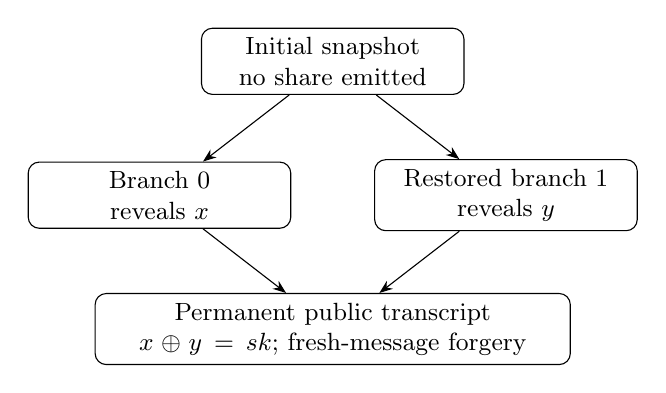
\begin{tikzpicture}[>=Stealth,
 b/.style={draw,rounded corners,align=center,text width=31mm,font=\small}]
\node[b] (snap) at (0,0) {Initial snapshot\\no share emitted};
\node[b] (a) at (-2.2,-1.7) {Branch 0\\reveals $x$};
\node[b] (bb) at (2.2,-1.7) {Restored branch 1\\reveals $y$};
\node[b,text width=58mm] (union) at (0,-3.4) {Permanent public transcript\\$x\oplus y=sk$; fresh-message forgery};
\draw[->] (snap)--(a);\draw[->] (snap)--(bb);
\draw[->] (a)--(union);\draw[->] (bb)--(union);
\end{tikzpicture}
\caption{A counterexample to the converse frozen-state implication. Each branch reveals one share that is individually independent of the secret key, but restoration does not erase the adversary's earlier observations. LULA I's honest caches avoid this mechanism by preserving one signing function.}\label{fig:branches}
\end{figure}

Each frozen initial signer is the base signer without a share. Each frozen absorbing signer reveals only one share, which is independent of $sk$ and can be simulated. A sequential path reveals at most one share. An adversary can instead snapshot the initial state, enter branch 0 and obtain $x$, restore, enter branch 1 and obtain $y$, recover $sk=x\oplus y$, and sign a fresh message. This is a conditional cryptographic counterexample built from any secure base scheme. Independent finite project controls exhibit the same branch-combination failure with hash-based authorization. Neither construction attacks LULA I, whose honest caches preserve one common function.

\section{Cache-accelerated signing}\label{sec:cache}
\Cref{fig:dependency} separates the source of authorization from its accelerated computations. The secret seed defines chain starts and FORS secrets; public addresses define their domains. The cache supplies previously computed nodes and counters. It supplies no trusted record of previously signed messages. The rollback unforgeability statement is conditional on an applicable bound for the common reference signer, as in \Cref{sec:security,thm:transfer}.

\begin{figure}[!htbp]
\centering
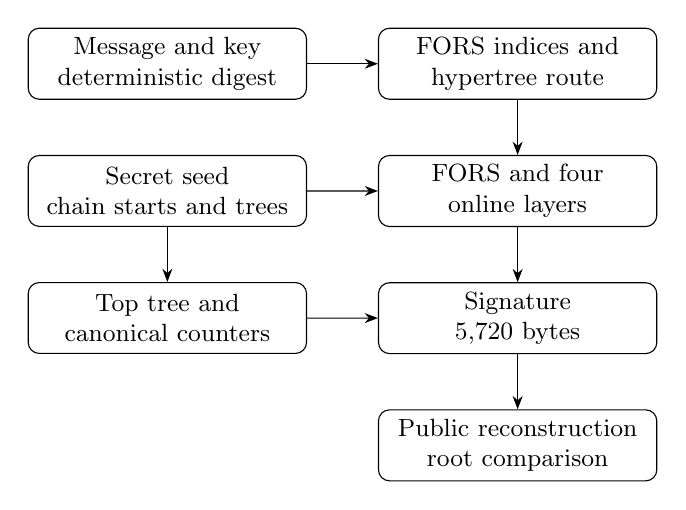
\begin{tikzpicture}[>=Stealth,node distance=7mm,
 box/.style={draw,rounded corners,align=center,font=\small,text width=33mm,minimum height=9mm}]
\node[box] (m) {Message and key\\deterministic digest};
\node[box,right=9mm of m] (route) {FORS indices and\\hypertree route};
\node[box,below=of m] (sk) {Secret seed\\chain starts and trees};
\node[box,below=of route] (online) {FORS and four\\online layers};
\node[box,below=of sk] (cache) {Top tree and\\canonical counters};
\node[box,below=of online] (sig) {Signature\\5,720 bytes};
\node[box,below=of sig] (vf) {Public reconstruction\\root comparison};
\draw[->] (m)--(route);\draw[->] (route)--(online);
\draw[->] (sk)--(online);\draw[->] (sk)--(cache);
\draw[->] (online)--(sig);\draw[->] (cache)--(sig);
\draw[->] (sig)--(vf);
\end{tikzpicture}
\caption{LULA I's dependency graph. Authorization follows the secret-derived objects and public verification. The cache accelerates fixed computations; removing the honest cache preserves signature bytes whenever signing terminates, but adds top-tree reconstruction and search.}\label{fig:dependency}
\end{figure}

The top cache contains $(2^{22}-1)$ nodes and $2^{21}$ counters. Its payload is exactly
\begin{equation}\label{eq:cache}
 C_{\mathrm{bytes}}=16(2^{22}-1)+4\cdot2^{21}
 =75{,}497{,}456\ \mathrm{bytes}.
\end{equation}
This is $72$ MiB minus 16 bytes. It excludes allocation headers, spare vector capacity, context, and temporary preparation buffers. A historical peak working-set observation was 122,384,384 bytes, approximately 116.71 MiB. Peak working set is an operating-system measurement, not the size of serialized cache payload.

There is no cache age variable in the implemented signer. An older honest prepared snapshot is just a copy of the same cache. A seed-only backup permits reconstruction but carries none of its computational acceleration. Missing top-layer state triggers full top-tree recomputation for the next signature; the library does not automatically rebuild and persist the cache after this operation.

Read-only cache copies also permit concurrent deterministic computations at the algorithmic level. The publication does not evaluate concurrent execution, crash consistency, deployment isolation, or a multi-device leakage model. Independent correctness of copied cache data is not a concurrency performance guarantee.

\section{Signing-query reference points, wire format and computation}\label{sec:cost}
% TODO(author): complete reference-signer operating-point derivation; the component coverage model is not a signing-capacity certificate.
\subsection{Signing-query reference points and a coverage model}\label{sec:operating}
The author-selected conditional use objective for the fixed LULA I parameter set is $q_{\mathrm{sig}}=2^{40}$ signing queries across all restored branches. It is not a certified signing capacity: the full reference-signer bound remains open. \Cref{tab:security-model} distinguishes this objective, published SLH-DSA query targets, and additional analytical scenarios.

The model considers a generic classical FORS coverage attack, following the occupancy analysis of Fluhrer and Dang~\cite[Section~5, Equation~(1)]{fluhrer}. It assumes independent uniform address and tree-index selections. For LULA I, with $\rho=2^{-41}$, $r=1-2^{-9}$ and $N$ exposures at one address, coverage of the 17 real trees has probability $(1-r^N)^{17}$. A raw candidate must also satisfy the nine-bit zero condition. Expanding the power gives
\[
 p_{\mathrm{raw}}=2^{-9}\sum_{j=0}^{17}(-1)^j\binom{17}{j}\,\mathbb E[r^{jN}].
\]
For Binomial occupancy, $N\sim\mathrm{Bin}(q_{\mathrm{sig}},\rho)$ and $\mathbb E[r^{jN}]=(1-\rho+\rho r^j)^{q_{\mathrm{sig}}}$. The Poisson approximation uses $\lambda=q_{\mathrm{sig}}\rho$ and $\mathbb E[r^{jN}]=\exp(\lambda(r^j-1))$. Both evaluations agree at the displayed precision for LULA I. The other rows apply the same Poisson occupancy method to their published FORS parameters, without LULA I's extra zero condition.

\begin{table}[!htbp]
\caption{Classical FORS coverage-model exponent $-\log_2 p_{\mathrm{raw}}$ per raw digest candidate, at the query count in the first column. LULA I includes its nine-bit forced condition (FORS+C). These derived component exponents are neither measured attacks nor full-signature security bounds. Independent uniform selections are premises; the LULA I hypertree term and full reference-signer bound remain open. S: source; D: derived; P: unestablished premise.}\label{tab:security-model}
\centering\small\setlength{\tabcolsep}{3pt}
\begin{tabular}{P{12mm}P{31mm}rP{43mm}}\toprule
$q_{\mathrm{sig}}$ & Construction & Exponent & Query-count status\\\midrule
$2^{24}$\textsuperscript{D} & LULA I\textsuperscript{S} &178.4\textsuperscript{D}&Model scenario\textsuperscript{D}\\
$2^{30}$\textsuperscript{D} & LULA I\textsuperscript{S} &167.8\textsuperscript{D}&Model scenario\textsuperscript{D}\\
$2^{38}$\textsuperscript{D} & LULA I\textsuperscript{S} &143.3\textsuperscript{D}&Model scenario\textsuperscript{D}\\
$2^{40}$\textsuperscript{S} & LULA I\textsuperscript{S} &132.6\textsuperscript{D}&Author's conditional objective\textsuperscript{S/P}\\
$2^{41}$\textsuperscript{D} & LULA I\textsuperscript{S} &125.9\textsuperscript{D}&Model scenario\textsuperscript{D}\\
$2^{42}$\textsuperscript{D} & LULA I\textsuperscript{S} &118.1\textsuperscript{D}&Model scenario\textsuperscript{D}\\
$2^{44}$\textsuperscript{D} & LULA I\textsuperscript{S} &98.5\textsuperscript{D}&Model scenario\textsuperscript{D}\\
$2^{50}$\textsuperscript{D} & LULA I\textsuperscript{S} &20.1\textsuperscript{D}&Model scenario\textsuperscript{D}\\
$2^{56}$\textsuperscript{D} & LULA I\textsuperscript{S} &9.0\textsuperscript{D}&Model scenario\textsuperscript{D}\\
$2^{64}$\textsuperscript{D} & LULA I\textsuperscript{S} &9.0\textsuperscript{D}&Model scenario\textsuperscript{D}\\\midrule
$2^{24}$\textsuperscript{S} & Draft SHA2-128-24\textsuperscript{S} &128.6\textsuperscript{D}&Published draft target\textsuperscript{S}\\
$2^{30}$\textsuperscript{D} & Draft SHA2-128-24\textsuperscript{S} &95.9\textsuperscript{D}&Scenario beyond draft target\textsuperscript{D}\\
$2^{40}$\textsuperscript{D} & Draft SHA2-128-24\textsuperscript{S} &36.1\textsuperscript{D}&Scenario beyond draft target\textsuperscript{D}\\
$2^{64}$\textsuperscript{D} & Draft SHA2-128-24\textsuperscript{S} &0.0\textsuperscript{D}&Scenario beyond draft target\textsuperscript{D}\\\midrule
$2^{24}$\textsuperscript{D} & SHA2-128s\textsuperscript{S} &207.0\textsuperscript{D}&Model scenario\textsuperscript{D}\\
$2^{30}$\textsuperscript{D} & SHA2-128s\textsuperscript{S} &201.0\textsuperscript{D}&Model scenario\textsuperscript{D}\\
$2^{40}$\textsuperscript{D} & SHA2-128s\textsuperscript{S} &191.0\textsuperscript{D}&Model scenario\textsuperscript{D}\\
$2^{64}$\textsuperscript{S} & SHA2-128s\textsuperscript{S} &133.7\textsuperscript{D}&Published parameter target\textsuperscript{S}\\\midrule
$2^{24}$\textsuperscript{D} & SHA2-128f\textsuperscript{S} &240.0\textsuperscript{D}&Model scenario\textsuperscript{D}\\
$2^{30}$\textsuperscript{D} & SHA2-128f\textsuperscript{S} &233.9\textsuperscript{D}&Model scenario\textsuperscript{D}\\
$2^{40}$\textsuperscript{D} & SHA2-128f\textsuperscript{S} &218.3\textsuperscript{D}&Model scenario\textsuperscript{D}\\
$2^{64}$\textsuperscript{S} & SHA2-128f\textsuperscript{S} &131.4\textsuperscript{D}&Published parameter target\textsuperscript{S}\\\bottomrule
\end{tabular}
\smallskip\par\raggedright\footnotesize SHA2-128s/128f denote the SLH-DSA-SHA2 parameter sets in FIPS~205~\cite{fips205}; SHA2-128-24 is the SP~800-230 initial public draft set~\cite[Table~1 and Section~3]{sp800230}, not a final standard or a measured campaign row. Selection assumptions are premises\textsuperscript{P}; a source target does not prove the same security for an auxiliary implementation. The displayed LULA I exponent conditional on an accepted candidate would be nine less. Entries rounded to 9.0 or 0.0 are not exact equalities at finite query counts. A component exponent above 128 does not establish 128-bit security for the whole signature scheme.
\end{table}

The LULA I raw-candidate exponent crosses 128 near $q_{\mathrm{sig}}=2^{40.7014}$ (approximately $1.788\cdot10^{12}$ queries) under this model. This numerical crossing is not a full reference-signer security threshold or a certified signing capacity. The exponent decreases by about 34.0 between $2^{40}$ and $2^{44}$ queries and approaches nine as coverage saturates. The author-selected conditional objective remains $2^{40}$; the other rows are analytical scenarios for the same parameters.

This model does not establish the assumed selection distributions for the complete deterministic signer or account for every forgery strategy, adversarial hash-query budget, hash derivation and hypertree obligation. It therefore supplies neither a security-normalized ranking nor a capacity certificate. The construction and measured parameter set are unchanged.

\FloatBarrier

\subsection{Exact wire format}
\Cref{tab:wire} gives every transmitted field in order. The parameter set is fixed externally and no parameter identifier is included in the signature. This is acceptable for a fixed-parameter interface but requires an explicit protocol identifier when integrating multiple schemes.

\begin{table}[t]
\caption{LULA I signature serialization. Offsets are zero based; counters are 32-bit big-endian integers. No message, public key, or padding is included in the signature.}\label{tab:wire}
\centering\small
\begin{tabular}{P{49mm}rr}\toprule
Field & Offset & Bytes\\\midrule
Randomizer $R$ &0&16\\
FORS+C counter $c_F$ &16&4\\
17 FORS secrets and nine-node paths &20&2720\\
Layer 0: counter, 32 values, 5 siblings &2740&596\\
Layer 1: counter, 32 values, 5 siblings &3336&596\\
Layer 2: counter, 32 values, 5 siblings &3932&596\\
Layer 3: counter, 32 values, 5 siblings &4528&596\\
Layer 4: counter, 16 values, 21 siblings &5124&596\\\midrule
Total &&5720\\\bottomrule
\end{tabular}
\end{table}

The size follows directly from the loops in \Cref{alg:sign}:
\begin{align}\label{eq:size}
 |\sigma|&=16+4+16\cdot17(9+1)
      +\sum_{j=0}^{4}(4+16\ell_j+16h_j)\nonumber\\
 &=16+4+2720+5\cdot596=5720\ \mathrm{bytes}.
\end{align}
Each layer happens to occupy 596 bytes for this set: the top layer trades 16 fewer chain values for 16 more path nodes. This equality does not hold for arbitrary parameter sets.

\subsection{Verification accounting}
Let $b(x)=\lceil(x+9)/64\rceil$ be the number of SHA-256 blocks for an $x$-byte suffix after a prepared 64-byte prefix. A WOTS public-key compression costs $b(22+16\ell_j)$ additional compressions. Chain completion costs $\ell_j(w_j-1)-S_j$, which is constant for accepted digit vectors.

For a 32-byte message, \Cref{tab:work} sums to 3,265 instrumented compressions. The implementation creates the public context with one additional prefix compression using an uncounted direct compression call. Including this initialization, valid verification executes 3,266 SHA-256 compressions. Hash calls and compression calls are different units: a single hash invocation can process several blocks.

\begin{table}[t]
\caption{Valid-signature verification work for a 32-byte message. The historical counter excludes context-prefix initialization. Malformed signatures may reject early.}\label{tab:work}
\centering\small
\begin{tabular}{P{61mm}r}\toprule
Operation & Compressions\\\midrule
Message inner hash and outer digest &3\\
FORS leaves, paths, and root compression &175\\
Four lower WOTS+C reconstructions and paths &1020\\
Top WOTS+C reconstruction and path &2067\\\midrule
Instrumented total &3265\\
Prefix-context initialization &1\\\midrule
Executed total &3266\\\bottomrule
\end{tabular}
\end{table}

This verification decomposition is derived from the implementation. For message length $L$, the instrumented verification count is $3263+\lceil(L+57)/64\rceil$. Signing also hashes $SK.prf\|PK.seed\|M$, costing $\lceil(L+41)/64\rceil$ blocks. Unbounded message length is incompatible with a universal fixed signing or verification latency bound.

\subsection{Prepared signing and search tails}
Let $G_F(M)$ count outer digest trials up to the first FORS+C acceptance, including the accepted trial. Let $G_j(M)$ count WOTS+C digest trials at uncached layer $j$, also including the accepted trial. For a 32-byte message, the following work decomposition is derived from the implementation and confirmed by the retained counter JSON:
\begin{equation}\label{eq:signwork}
 W_{\mathrm{hot}}(M)=96{,}082+G_F(M)+\sum_{j=0}^{3}G_j(M).
\end{equation}
The fixed term includes 26,117 FORS compressions, four reconstructed height-5 trees, chain signing, digest checks after searching, and top-layer signing. The top counter search is paid during preparation. The FORS decomposition, derived from the implementation, is $17(512+512+511+1)+5=26{,}117$: each tree has secret derivations, leaf hashes, inner hashes, and one selected-secret rederivation; root compression costs five blocks. With the child-tree count below, the fixed term is
\[
 4+26{,}117+4(16{,}703+32+240+1)+16+2040+1=96{,}082.
\]
The four initial blocks compute the randomizer and inner digest for a 32-byte message. Each lower layer adds its tree, 32 secret derivations, 240 chain steps and one accepted-digest recomputation. The last terms derive and sign the top key and recompute its accepted digest. Search trials remain in $G_F$ and $G_j$.

For an idealized unbounded sequence of independent uniform candidate digests, the trial-count proxy for $G_F$ is geometric with success probability $2^{-9}$. At layer $j$, let $\nu_j=[x^{S_j}](1+x+\cdots+x^{w_j-1})^{\ell_j}$. Its search success probability is $p_j=\nu_j/w_j^{\ell_j}$. The unbounded geometric proxy has mean $1/p_j$ and tail $(1-p_j)^t$.

The tail law describes executable trials only while counters remain distinct, with $t\le 2^{32}$. Under the independence premise, the event that all $N=2^{32}$ candidates are rejected has probability $(1-p_j)^N$; this model does not establish that every executable search terminates. A confidence budget split among all five online searches gives a probabilistic work quantile through a union bound. It does not give certified worst-case time.

The recovered analytical script reports expected prepared signing near 96,858 instrumented compressions and a heuristic $2^{-30}$ tail value near 112,189. Under the same uniform search model, its expected-signing formula counts one extra outer-trial compression relative to the source-exact mean from \Cref{eq:signwork}. Its shared-tail approximation is retained as a historical model rather than a validated joint-tail certificate. The measured maximum of 100,586 instrumented compressions is simply the largest value in one recorded sample.

\subsection{Preparation and missing-cache cost}
The historical preparation counter records approximately $2^{35.396}$ compressions, including both key setup and cache construction; it reports the logarithm rounded to three decimals. This is neither an exact universal setup count nor a worst-case bound on all canonical searches.

Derived from the implementation, one top-layer WOTS public key costs $16\cdot255+16+5=4101$ counted compressions: 16 chains of 255 steps, 16 secret derivations, and five blocks for public-key compression. Recomputing the height-21 subtree costs
\[
 2^{21}\cdot4101+(2^{21}-1)=8{,}602{,}517{,}503
\]
counted compressions, before the other signing work and the top counter search. A recorded absent-cache signature used 8,602,614,065 counted compressions. The arithmetic identifies the cause of the cold penalty independently of any elapsed-time measurement.

Under the idealized unbounded independent-trial search model, preparation's expected executed cost, including its initially uncounted prefix block, is
\[
 2^{21}\left(4101+16{,}703+\frac{1}{p_4}+1\right).
\]
Derived from the implementation, $16{,}703=32\cdot521+31$ is the height-5 child-tree work: 32 WOTS public keys of $32\cdot15+32+9=521$ compressions, and 31 inner-node hashes. The recovered expected-cost model differs by $2^{22}$ compressions from this source-exact expression, although its rounded exponent remains close. The analytical setup model therefore does not match the executable count exactly.

\section{Implementation}\label{sec:implementation}
The evaluated library is Rust, with \texttt{sha2} version 0.10.9 and its compression feature. Release settings use optimization level 3, one code-generation unit, link-time optimization, and no debug information. Nodes are fixed-size byte arrays; counters and subtrees are held in vectors. Hash work is recorded in a thread-local counter.

The original key-generation harness can split work over threads. Recorded full-parameter preparation used 12 workers, whereas signing and verification used one pinned thread. Preparation times from that harness must not be described as single-core key-generation measurements. The mathematical algorithms do not require multicore execution.

% TODO(author,Q5): identify each historical timed binary and bind it to its source/build inputs; do not infer correspondence from a later rebuild.
One historical timing binary preceded the source's explicit cached-counter acceptance guard. Honest cache outputs agree, but the historical executable is not fully bound to the publication snapshot by a recorded build digest. Its timings are retained as historical evidence, rather than as measurements of a newly rebuilt binary.

An independently written Python verifier reconstructs addresses, paths, digit sums, and serialization from the project specification. It accepted all 12 historical known-answer vectors across four parameter sets, including three for the main LULA I set. For each vector, it rejected a changed message and a changed signature. Independence here means a separate implementation of the stated specification, not independent cryptanalysis.

For the publication replay, a new driver used the unchanged library snapshot, pinned its process to logical CPU 0, and requested BelowNormal priority. It performed 1,000 full-parameter verifications on one recovered 32-byte-message fixture, plus 64 cache-present/cache-absent/cache-restored comparisons on a small two-layer correctness configuration. The small set is explicitly not the LULA I security parameter set. A dedicated control altered a top-layer counter to the next accepted counter and checked that the resulting signature was different but accepted.

The source has no general parameter-validation API, persistent cache codec, explicit search-overflow contract, or memory-integrity protocol. The fixed parameter set avoids digest-index overflow, but a caller supplying arbitrary parameters can trigger invalid indexing or assertions. The research library is not presented as a hardened production signing service.

\section{Historical measurements and publication replay}
This section reports historical sessions and the fixed-fixture publication replay. The first campaign and gated follow-up remain separate execution records in \Cref{sec:benchcomparison,sec:stability}.\label{sec:experiments}
\subsection{Methodology and environment}
All reported times are elapsed latencies in milliseconds unless explicitly stated otherwise. Historical sessions used an Intel Core Ultra 7 255U and Windows 11; the recorded Rust toolchain is 1.97.1. The full-parameter harness pinned its benchmark thread to affinity mask 16 and requested highest thread priority. Foreign workloads varied between sessions. Message fixtures were 32 bytes; their deterministic generator was used for reproducibility, not cryptographic randomness.

The publication replay verified the same CPU model and Rust 1.97.1 on an x86-64 Windows MSVC target, with one process-affinity bit and BelowNormal priority. The dependency supports runtime hardware dispatch; SHA acceleration was not separately disabled and reenabled in this replay, so no backend speedup is attributed. Processor frequency, thermal state, the full set of concurrent external workloads, and scheduling interruptions affecting individual samples were not controlled. Maxima include operating-system delays. The replay is correctness and latency evidence under the measured environment, not a worst-case execution certificate.

\begin{table}[!htbp]
\caption{Evidence class and execution context. CPU indices are logical processors. Counts are timed calls per operation, not independent keys; historical and replay data are separate from either campaign.}\label{tab:execution-contexts}
\centering\scriptsize\setlength{\tabcolsep}{2pt}
\begin{tabular}{P{18mm}P{8mm}P{19mm}P{20mm}P{23mm}P{21mm}}\toprule
Record & CPU & Priority & Load sampling & Binary identity & $N$ per cell\\\midrule
Historical sessions & 4 & Highest thread & Varying workloads & Not bound & 2,000 / 1,000 / 200; cold 1\\
Publication replay & 0 & BelowNormal & Recorded environment & Timed binary not bound & 1,000 verifies\\
First campaign & 10 & BelowNormal & Job endpoints & D1, D3--D6 & L/F: 1,000; S: 100; SF: 200; FB/R: 20; G: 12\\
Gated follow-up & 10 & BelowNormal & Continuous, about 1 Hz; preceding-window gate & D1--D3 & L/F: 1,000/block; S: 200/block; six blocks\\
\bottomrule\end{tabular}
\smallskip\par\raggedright\footnotesize The first-campaign counts shown are its 32-byte overview cells. Other input lengths and recovery counts are retained in their detailed tables. L/F/S denote LULA I/SHA2-128f/SHA2-128s; SF/FB denote upstream C B32 stateful/fallback; R/G denote the C reconstruction/third-party Go adapter. Recorded first-campaign and follow-up jobs share a 2.75 GiB per-process ceiling; siblings, instantaneous frequency and temperature were not physically controlled. D1--D6 are listed below; D4--D6 identify the auxiliary overview binaries.
\end{table}

\FloatBarrier

The recorded SHA-256 identities used above are D1 (LULA I key-1 driver), D2 (LULA I seed-configurable driver), D3 (OpenSSL adapter), D4 (upstream C B32), D5 (C compact reconstruction), and D6 (third-party Go adapter). They are listed in two consecutive 32-hexadecimal-character halves for readability:
\begin{center}\scriptsize\ttfamily
\begin{tabular}{lll}
D1 & 020e94beeb18e7f17ae87345120cbe92 & be929acbd47c415c505ecaa9bf5a4d31\\
D2 & d6bb7b4e0dd75d299607151aa420fcc6 & 709583b3dd9ac9db58b4e0b3884681c1\\
D3 & 612ed160dbbfe470a8bb6e0122318fbb & 5701c8ae292dafaddf0a4ee4eb35676e\\
D4 & 5be466a191c84b436bfec94882a0f5ee & 82c5054b87403e6642664e45c4fed812\\
D5 & eb88874743056a0aa02b4f8239cd6889 & d161e8af052a64c1415fc9d4c4dd5bb7\\
D6 & a20a86ddbd1d8454c957b22252c7bd13 & beada5f6c326739f630306341f52f5a5\\
\end{tabular}\end{center}
These identify the primary and auxiliary comparison binaries. A source snapshot or a later rebuild does not bind an earlier timed binary.

Historical sessions denote retained prior harness runs; publication replay denotes the isolated fixed-fixture reconstruction; campaign denotes each separately frozen implementation experiment. The first campaign sampled load at endpoints; the gated follow-up used a preceding-window gate and continuous sampling. \Cref{tab:execution-contexts} keeps these contexts distinct. Historical prepared-signing medians of 5.6--9.5 ms and the first campaign's 3.9--4.6 ms are different executions; their difference is not attributed to a cause.

Historical aggregate files preserve sample counts, selected quantiles, and maxima, but not every raw repetition. Their p95 values cannot be reconstructed without fabricating a distribution. The new fixed-fixture replay preserves every raw verification duration and uses the nearest-index quantile rule with index $\operatorname{round}((N-1)p)$; Rust half-integer ties round upward. Historical timings use the historical driver's own implementation of that rule.

\subsection{Recorded full-parameter lifecycle}
\Cref{tab:history} preserves complete rows within their individual runs. The session rows report the first signing and verification measurements for each message. A separate statistic taking the minimum over six attempts for each message reports its fastest observed attempt; it does not describe the latency of a randomly selected attempt.

\begin{table}[t]
\caption{Historical sessions: full-parameter elapsed measurements in milliseconds. Each row is a separate scenario; unavailable p95 values are not inferred. Prepared and restored rows in the lifecycle run use 200 messages.}\label{tab:history}
\centering\small
\begin{tabular}{P{37mm}rrrrr}\toprule
Scenario & $N$ & Min & Median & p99 & Max\\\midrule
Session A signing &2000&7.531&8.629&10.184&19.063\\
Session A verification &2000&0.258&0.290&0.362&17.074\\
Session B signing &1000&3.663&5.633&7.596&9.127\\
Session B verification &1000&0.122&0.194&0.267&1.486\\
Lifecycle prepared &200&9.025&9.452&18.720&21.223\\
Lifecycle restored &200&9.043&9.975&12.791&14.749\\
Lifecycle absent &1&\multicolumn{4}{c}{703,995.742 ms; byte-identical output}\\\bottomrule
\end{tabular}
\end{table}

Initial prepared setup took 990.62 seconds in session A and 383.01 seconds in session B, both with 12 workers. In the lifecycle run it took 838.60 seconds. A later full rebuild under saturation took 14,031.05 seconds. Setup and rebuild times include cache construction, not only the minimum computations necessary to establish the public root.

The absent-cache observation of 703.996 seconds and the earlier observation of 689.423 seconds concern the same parameter set in different runs. Both produced the same output bytes as their cached counterparts. Their difference is not a change in the mathematical construction.

\subsection{Publication replay and negative controls}
\begin{table}[t]
\caption{Publication replay: one full-parameter 32-byte-message fixture, 1,000 valid verifications, logical CPU 0 and BelowNormal priority. All raw durations are retained; no selected minimum over repetitions is used.}
\label{tab:replay}
\centering\small
\begin{tabular}{lrrrrr}\toprule
Operation & Min & Median & p95 & p99 & Max\\\midrule
Verification (ms) & 0.1334 & 0.1360 & 0.1465 & 0.1847 & 0.8732\\\bottomrule
\end{tabular}
\end{table}
\Cref{tab:replay} reports the final run, which retained every raw duration. An earlier exploratory execution recorded a 33.069 ms verification maximum; its aggregate is also preserved. The rerun added raw-duration retention without establishing a new latency guarantee. Neither sample certifies a worst-case elapsed-latency bound.

The replay's fixed full-parameter fixture was verified 1,000 times. Every successful verification recorded 3,265 instrumented compressions. Eight bit flips across serialized fields and two nonexact-length signatures were rejected. The same fixture was used repeatedly, so this sample is not a distribution over independently selected messages.

Across 64 distinct four-byte messages in the miniature configuration, prepared, deleted, and restored caches yielded identical bytes. These tests complement \Cref{lem:transparent}; their finite success does not prove a security level. The arbitrary-write control found a second accepted counter and produced a different accepted signature on the same message, exposing the gap between honest restoration and corrupted-cache handling.

The restored-generator control uses 22 digest-selection bits in a toy hash-based construction. With the randomizer known before selecting the next messages, its birthday search found a colliding pair in 2,712 hash trials, after which a signature on one message verified for the other. The same attack did not forge its fresh-entropy or deterministic message-dependent controls. Failure of those bounded attacks is not a proof that the controls are secure.

The random-start cached-counter control obtained six different accepted digests at one upper WOTS address and forged after eight counter trials. The smallest-counter control emitted one digest and resisted that particular search through $2^{20}$ attempts. This bounded toy control isolates how noncanonical counter selection changes the evidence exposed at one address.

The historical 720 restoration schedules cover an abstract toy-family comparison. Full-parameter evidence includes known-answer verification and a limited number of cache-loss byte comparisons. The finite controls demonstrate particular state-transition mechanisms; they do not replace the transcript proof or its assumptions.

\subsection{Competing explanations for performance}
Three possible explanations for performance improvements are parameterization, preprocessing and caching, and implementation optimization. Holding the parameter set, message, code, and output fixed while disabling the cache distinguishes the contribution of preprocessing from a purely parameter-based explanation. The cold-tree work count independently explains why that intervention is expensive. Historical cached versus uncached signatures support a large preprocessing contribution for this specific parameter set.

The different-layer widths change signature size and verification work analytically, supporting the existence of a parameter tradeoff, but the available measurements do not isolate the contribution of parameterization to the observed signing and verification latency differences. Those observations concern the fixed parameter set at the conditional $2^{40}$-query use objective, with an unresolved full reference bound (\Cref{sec:operating}); they establish no common-security advantage. Similarly, SHA dispatch, compiler settings, vectorization, and scheduling can affect elapsed latency, but no completed controlled backend ablation isolates the contribution of implementation optimization here. No comparative dominance is inferred from a faster median on a different machine or from a minimum selected across repetitions.

\section{Gated follow-up evaluation}\label{sec:stability}
\subsection{Design and observed workload control}
A separate follow-up campaign tested the repeatability of the principal implementation comparison in \Cref{sec:benchcomparison}. It ran on the same physical host and logical processor 10, at BelowNormal priority, with the same 2.75 GiB memory ceiling. The key-1 LULA I and OpenSSL adapter executables match the earlier campaign's recorded SHA-256 digests. A seed-configurable LULA I driver prepared a second fixture key. The hardware and reused binaries were held fixed, while background activity changed; differences between campaigns are not a controlled speedup.

Six blocks covered three message lengths and three implementations. LULA I alternated two fixture keys, with three blocks per key; OpenSSL generated a new key per process and used its default hedged mode. LULA I signing was deterministic. Each LULA I and SHA2-128f block retained 1,000 signing and 1,000 verification calls; SHA2-128s retained 200 each. Job order was shuffled with seed $20261012+b$ in block $b$, and inter-block gaps were at least three minutes. The full campaign comprised 54 prepared-comparison jobs, 15 fresh-process jobs and three cache-loss jobs. All 72 completed with exit code zero. Repeated schedules and fixture keys do not constitute independently sampled messages and keys on every call.

Before each job, the controller required at least three sampler rows from the preceding 20 seconds, with mean total CPU busy time at most 30\% and mean busy time of logical processors 10 and 11 at most 8\% each. The final gate log contains 176 decisions: 72 passes and 104 waiting records, with no timeout. All passing windows were independently recomputed. Failed attempts were logged periodically, rather than at every retry. The final controller has no separate five-second settle delay; the preceding-window gate is the implemented procedure.

The replacement sampler records CPU busy-time fractions from system counters, not frequency-scaled processor utility. Its 12,737 rows have a median interval of 1.000777 seconds and a maximum interval of 2.010287 seconds. Process names were not collected. A job is flagged as contaminated if its process interval contains fewer than three rows, its mean logical-11 busy time exceeds 15\%, or its mean total busy time exceeds 45\%. None was flagged. The largest job means were 6.533\% for logical 11 and 14.492\% for the total. Within job intervals, individual sibling samples reached 31.2\%; the sibling was monitored, not physically isolated. Whole-process means include loading and may dilute brief contention. Whole-second process timestamps also limit alignment with sampler intervals. Reported frequency values do not establish fixed instantaneous frequency; temperature and throttling remained uncontrolled.

\subsection{Latency distributions and block stability}
We recomputed every elapsed statistic from retained integer nanoseconds. Medians use the midpoint of the two central observations for even $N$; percentiles use nearest rank. \Cref{tab:stability-latencies} pools retained blocks while \Cref{tab:stability-verdicts} preserves their variation. Negative-control sentinels are untimed and excluded. Sample counts denote timed calls, not independent experiments. Every maximum is an observed maximum.

\begin{table}[t]
\caption{Follow-up elapsed latencies and between-block variation. Times are milliseconds; spread is the range of the six block medians divided by their mean, in percent. L: prepared LULA I; F/S: OpenSSL SHA2-128f/128s; S/V: signing/verification. Each median and its spread appear in the same row. Query points: LULA I conditional $2^{40}$; SLH-DSA published $2^{64}$ (\Cref{tab:security-model}). Max is the maximum observed latency, not a bound.}\label{tab:stability-latencies}
\centering\small\setlength{\tabcolsep}{2pt}
\begin{tabular}{llrrrrrrr}\toprule
Cell & Op. & $N$ & Min & Median & Spread (\%) & p95 & p99 & Max\\\midrule
% b1 source: STABILITY-FINDINGS.md line 13; exact fields recomputed from CSV/raw, T05_SOURCE_MAP.json.
L/32 B & S & 6000 & 3.4447 & 3.5917 & 4.20 & 4.1308 & 6.3176 & 57.2617\\
% b1 source: STABILITY-FINDINGS.md line 14; exact fields recomputed from CSV/raw, T05_SOURCE_MAP.json.
L/32 B & V & 6000 & 0.1169 & 0.1186 & 1.27 & 0.1302 & 0.2040 & 1.8697\\
% b1 source: STABILITY-FINDINGS.md line 15; exact fields recomputed from CSV/raw, T05_SOURCE_MAP.json.
L/1 KiB & S & 6000 & 3.4472 & 3.5610 & 1.41 & 4.0184 & 4.9656 & 26.2367\\
% b1 source: STABILITY-FINDINGS.md line 16; exact fields recomputed from CSV/raw, T05_SOURCE_MAP.json.
L/1 KiB & V & 6000 & 0.1173 & 0.1194 & 0.92 & 0.1290 & 0.2633 & 4.5739\\
% b1 source: STABILITY-FINDINGS.md line 17; exact fields recomputed from CSV/raw, T05_SOURCE_MAP.json.
L/64 KiB & S & 6000 & 3.4972 & 3.6371 & 2.27 & 4.1355 & 5.6228 & 87.9172\\
% b1 source: STABILITY-FINDINGS.md line 18; exact fields recomputed from CSV/raw, T05_SOURCE_MAP.json.
L/64 KiB & V & 6000 & 0.1437 & 0.1453 & 0.86 & 0.1558 & 0.2703 & 9.7976\\
% b1 source: STABILITY-FINDINGS.md line 19; exact fields recomputed from CSV/raw, T05_SOURCE_MAP.json.
F/32 B & S & 6000 & 10.2578 & 10.7753 & 1.53 & 11.6389 & 16.9220 & 125.5747\\
% b1 source: STABILITY-FINDINGS.md line 20; exact fields recomputed from CSV/raw, T05_SOURCE_MAP.json.
F/32 B & V & 6000 & 0.5688 & 0.6311 & 1.80 & 0.7785 & 1.0835 & 91.7043\\
% b1 source: STABILITY-FINDINGS.md line 21; exact fields recomputed from CSV/raw, T05_SOURCE_MAP.json.
F/1 KiB & S & 6000 & 10.2615 & 10.8329 & 1.57 & 11.9904 & 20.1320 & 122.2416\\
% b1 source: STABILITY-FINDINGS.md line 22; exact fields recomputed from CSV/raw, T05_SOURCE_MAP.json.
F/1 KiB & V & 6000 & 0.5678 & 0.6326 & 3.55 & 0.8040 & 1.1071 & 113.7807\\
% b1 source: STABILITY-FINDINGS.md line 23; exact fields recomputed from CSV/raw, T05_SOURCE_MAP.json.
F/64 KiB & S & 6000 & 10.3319 & 10.8369 & 2.01 & 11.5689 & 15.9241 & 122.8180\\
% b1 source: STABILITY-FINDINGS.md line 24; exact fields recomputed from CSV/raw, T05_SOURCE_MAP.json.
F/64 KiB & V & 6000 & 0.6265 & 0.6909 & 1.74 & 0.8575 & 1.1457 & 115.9345\\
% b1 source: STABILITY-FINDINGS.md line 25; exact fields recomputed from CSV/raw, T05_SOURCE_MAP.json.
S/32 B & S & 1200 & 218.4715 & 232.1651 & 1.73 & 266.8282 & 330.2543 & 605.5695\\
% b1 source: STABILITY-FINDINGS.md line 26; exact fields recomputed from CSV/raw, T05_SOURCE_MAP.json.
S/32 B & V & 1200 & 0.1975 & 0.2295 & 2.07 & 0.2663 & 0.4604 & 0.8000\\
% b1 source: STABILITY-FINDINGS.md line 27; exact fields recomputed from CSV/raw, T05_SOURCE_MAP.json.
S/1 KiB & S & 1200 & 218.8560 & 231.7642 & 1.64 & 264.7282 & 324.0112 & 619.1274\\
% b1 source: STABILITY-FINDINGS.md line 28; exact fields recomputed from CSV/raw, T05_SOURCE_MAP.json.
S/1 KiB & V & 1200 & 0.1956 & 0.2278 & 2.81 & 0.2783 & 0.4940 & 1.5997\\
% b1 source: STABILITY-FINDINGS.md line 29; exact fields recomputed from CSV/raw, T05_SOURCE_MAP.json.
S/64 KiB & S & 1200 & 218.8485 & 231.1751 & 2.33 & 260.3025 & 312.0871 & 591.6050\\
% b1 source: STABILITY-FINDINGS.md line 30; exact fields recomputed from CSV/raw, T05_SOURCE_MAP.json.
S/64 KiB & V & 1200 & 0.2634 & 0.2968 & 1.75 & 0.3454 & 0.6498 & 10.9729\\
\bottomrule\end{tabular}
\end{table}

\begin{table}[t]
\caption{Six-block follow-up stability. Median ranges are milliseconds; spread is the block-median range divided by its mean. Tail ratio is the largest block p99/median. Key difference compares the medians of three block medians per LULA I fixture key, divided by their mean; it is descriptive and confounded with block time.}\label{tab:stability-verdicts}
\centering\small\setlength{\tabcolsep}{3pt}
\begin{tabular}{llrrrrl}\toprule
Cell & Op. & Median range & Spread (\%) & Tail ratio & Key (\%) & Verdict\\\midrule
L/32 B & S & 3.5173--3.6675 & 4.20 & 2.635 & 1.51 & stable\\
L/32 B & V & 0.1180--0.1195 & 1.27 & 2.383 & 0.25 & stable\\
L/1024 B & S & 3.5316--3.5818 & 1.41 & 1.778 & 0.90 & stable\\
L/1024 B & V & 0.1186--0.1197 & 0.92 & 2.516 & 0.42 & stable\\
L/65536 B & S & 3.5904--3.6729 & 2.27 & 2.609 & 0.30 & stable\\
L/65536 B & V & 0.1447--0.1460 & 0.86 & 2.353 & 0.62 & stable\\
F/32 B & S & 10.6979--10.8629 & 1.53 & 1.992 & -- & stable\\
F/32 B & V & 0.6265--0.6379 & 1.80 & 2.375 & -- & stable\\
F/1024 B & S & 10.7722--10.9428 & 1.57 & 2.371 & -- & stable\\
F/1024 B & V & 0.6217--0.6442 & 3.55 & 1.847 & -- & stable\\
F/65536 B & S & 10.7114--10.9288 & 2.01 & 1.596 & -- & stable\\
F/65536 B & V & 0.6861--0.6981 & 1.74 & 2.105 & -- & stable\\
S/32 B & S & 230.7503--234.7610 & 1.73 & 2.036 & -- & stable\\
S/32 B & V & 0.2268--0.2315 & 2.07 & 2.234 & -- & stable\\
S/1024 B & S & 229.7066--233.5138 & 1.64 & 1.450 & -- & stable\\
S/1024 B & V & 0.2253--0.2317 & 2.81 & 3.372 & -- & unstable\\
S/65536 B & S & 228.5634--233.9415 & 2.33 & 1.484 & -- & stable\\
S/65536 B & V & 0.2940--0.2993 & 1.75 & 3.426 & -- & unstable\\
\bottomrule\end{tabular}
\end{table}

The declared criterion requires at least four uncontaminated gated blocks, a block-median spread no greater than 5\% of its mean, and every block p99 no greater than three times that block's median. All six LULA I cells meet this criterion. SHA2-128s verification at 1 KiB and 64 KiB is \emph{unstable}: its largest block p99/median ratios are 3.372 and 3.426. These cells remain in the tables. Stable medians and p99 values do not constrain isolated maxima. \Cref{fig:stability-distributions} shows the pooled 32-byte distributions, including the observed tails.

\begin{figure}[!htbp]
\centering\includegraphics[width=\textwidth]{figures/stability-distributions.pdf}
\caption{Pooled empirical cumulative distributions of follow-up signing and verification on 32-byte messages, with logarithmic elapsed-time axes. LULA I uses a prepared cache. Query points are conditional $2^{40}$ for LULA I and published $2^{64}$ for SLH-DSA (\Cref{tab:security-model}). Curves retain observed tails across six gated blocks; their samples and backends differ, and no security-normalized ranking follows.}\label{fig:stability-distributions}
\end{figure}

\subsection{Recovery and independently checked output}
\Cref{tab:stability-recovery} reports fifteen fresh processes using key 1 and a 32-byte message. Loading and first signing are summed within each process before aggregation; OS process launch is excluded. Three cache-loss jobs each contain one recorded first signature in a separate process. Their individual durations are retained without fitting a recovery distribution from three points.

\begin{table}[!htbp]
\caption{Follow-up LULA I recovery on key 1 and 32-byte messages, in seconds. Fresh-process statistics use 15 processes. Each cache-loss row is one observed first signature; no three-point tail estimate is inferred.}\label{tab:stability-recovery}
\centering\small
\begin{tabular}{lrrrr}\toprule
Interval & $N$ & Min & Median & Max\\\midrule
Fresh process: cache load & 15 & 5.5610664 & 5.6962471 & 6.0908076\\
Fresh process: first Sign & 15 & 0.0035377 & 0.0035796 & 0.0038098\\
Paired load plus first Sign & 15 & 5.5646460 & 5.7000569 & 6.0943592\\
Cache loss, process 1 & 1 & \multicolumn{3}{c}{331.8369642}\\
Cache loss, process 2 & 1 & \multicolumn{3}{c}{337.5630796}\\
Cache loss, process 3 & 1 & \multicolumn{3}{c}{330.0493122}\\
\bottomrule\end{tabular}
\end{table}

The independent Python verifier accepted all 36 saved LULA I vectors and rejected the tested message-bit and signature-byte changes. Grouping by complete public key and message yields six groups, each with one distinct 5,720-byte signature. The key-1/32-byte group contains 21 vectors: three prepared, fifteen fresh and three cache-loss outputs. The other five groups contain three prepared outputs each. Cross-regime byte equality is therefore directly checked for key 1 at 32 bytes; this does not establish recovery coverage for key 2 or larger messages. The saved vectors are one retained output per LULA I job, not independent replay of every timed call.

Sixteen of the eighteen prepared-latency cells meet the declared stability criterion; the two SHA2-128s verification exceptions remain visible. This follow-up neither changes LULA I's unresolved reference-signer bound nor adds new SHRINCS or compact-adapter measurements. Compiler and hash backends remain unequal, and monitoring at roughly one-second resolution does not establish exclusive-core execution or a worst-case latency bound. The earlier campaign remains a separate record of behavior under its measured host activity.

\FloatBarrier

\section{First-campaign evaluation and implementation comparison}\label{sec:benchcomparison}
\subsection{Evidence cutoff and measurement boundaries}
The campaign recorded signing and verification latencies, initialization costs, and LULA I fixed-snapshot behavior. Its final retained record was frozen at 14:52 UTC on 12 October 2026. All four controllers have completion markers, and all 81 recorded processes completed with exit code zero. We independently checked the 477 retained file digests and recomputed distributions from 64 campaign CSV files, excluding smoke tests. Process completion establishes that scheduled jobs ended; it does not establish conformance or completion of the original experimental protocol. This first campaign lacked quiet-window trials, equivalent backends and a common-security cohort. The later workload gate and two-key prepared measurements are reported separately in \Cref{sec:stability}. The tables use raw observations subject to the inclusion criteria stated here, rather than relying on the campaign's summary labels.

The physical host was an Intel Core Ultra 7 255U with 32 GiB RAM running Windows 11 Pro, build 26300, under the Balanced power plan. Each measured campaign child job was pinned to logical processor 10 (affinity mask 1024), at BelowNormal priority, with a 2.75 GiB committed-memory ceiling. Its SMT sibling was not isolated. Other user workloads continued. The controller sampled system load before and after jobs, rather than continuously. CPU frequency and temperature were not controlled. Thus the experiment fixes a processor affinity but does not meet a quiet, isolated-core protocol.

LULA I used Rust 1.97.1 and \texttt{sha2} 0.10.9, with optimization level 3, one codegen unit and link-time optimization. The C adapters used Clang 22.1.8 with \texttt{-O3 -mno-avx}; OpenSSL 3.5.7 was supplied by the Git for Windows DLL and retained its runtime dispatch. Equivalent source-level flags do not make these hash backends equivalent, and instrumentation also differs. We report implementation observations; we do not attribute between-scheme timing differences solely to cryptographic design.

Elapsed nanoseconds were measured with high-resolution platform counters. Signing and verification were timed separately around individual API calls. Message construction and process launch are outside these intervals. The OpenSSL adapter initializes its API contexts before timing; internal hash-context initialization performed by a signing call remains inside that call's interval. The adapter supplies no deterministic-mode parameter, so OpenSSL uses its default randomized (hedged) signing mode~\cite{openssl}; LULA I signing is deterministic. OpenSSL uses the whole-message SLH-DSA interface with empty context~\cite{openssl}; the LULA I interface hashes the complete input internally. A 32-byte input is a raw digest-sized message, not a standardized prehash-mode measurement. No separate external-prehash cost was measured. LULA I uses replicates 0 through $N-1$, whereas the OpenSSL driver uses 1 through $N$; these are equal-length cells, not paired-message trials. LULA I uses one key throughout this campaign; OpenSSL generates one key per message-length cell.

The median is the midpoint of the two central order statistics when $N$ is even. Percentiles use nearest rank, $x_{\lceil pN\rceil}$ in one-based sorted order. This differs from the earlier verification replay's nearest-index convention. Untimed negative-control sentinels are excluded. We retain observed maxima and sample counts without interpreting them as mathematical runtime bounds.

\subsection{Prepared signing and whole-message verification}
\begin{table}[t]
\caption{First-campaign signing (S) and verification (V) elapsed latencies, in milliseconds. Signing-query reference points differ; see \Cref{sec:operating}. Max is the maximum observed, not a worst-case bound.}\label{tab:comparison-latencies}
\centering\small\setlength{\tabcolsep}{3pt}
\begin{tabular}{llrrrrrr}\toprule
Cell & Op. & $N$ & Min & Median & p95 & p99 & Max\\\midrule
L/32 B & S & 1000 & 4.151 & 4.600 & 5.332 & 5.718 & 30.530\\
L/32 B & V & 1000 & 0.129 & 0.141 & 0.166 & 0.190 & 5.629\\
L/1 KiB & S & 1000 & 3.676 & 3.920 & 4.242 & 4.843 & 12.162\\
L/1 KiB & V & 1000 & 0.125 & 0.131 & 0.142 & 0.179 & 0.279\\
L/64 KiB & S & 1000 & 3.685 & 3.968 & 4.696 & 5.249 & 10.778\\
L/64 KiB & V & 1000 & 0.151 & 0.161 & 0.189 & 0.228 & 0.388\\
F/32 B & S & 1000 & 10.522 & 12.004 & 14.181 & 21.761 & 44.068\\
F/32 B & V & 1000 & 0.615 & 0.719 & 0.847 & 1.024 & 3.913\\
F/1 KiB & S & 1000 & 12.011 & 13.925 & 18.339 & 25.634 & 36.288\\
F/1 KiB & V & 1000 & 0.684 & 0.823 & 1.018 & 1.549 & 2.744\\
F/64 KiB & S & 1000 & 10.642 & 11.498 & 13.626 & 16.378 & 383.005\\
F/64 KiB & V & 1000 & 0.659 & 0.741 & 0.897 & 1.084 & 17.350\\
S/32 B & S & 100 & 251.915 & 268.616 & 330.976 & 367.905 & 408.373\\
S/32 B & V & 100 & 0.234 & 0.268 & 0.321 & 0.362 & 0.500\\
S/1 KiB & S & 100 & 249.424 & 259.794 & 327.080 & 362.245 & 373.314\\
S/1 KiB & V & 100 & 0.228 & 0.262 & 0.311 & 0.380 & 0.429\\
S/64 KiB & S & 100 & 232.917 & 247.069 & 259.209 & 267.189 & 279.123\\
S/64 KiB & V & 100 & 0.290 & 0.319 & 0.358 & 0.436 & 0.446\\
\bottomrule\end{tabular}
\smallskip\par\raggedright\footnotesize L: prepared LULA I; F/S: OpenSSL SLH-DSA-SHA2-128f/128s. Message sizes refer to raw bytes supplied to the signing API. Values rounded to 0.001 ms; raw nanoseconds are retained.
\end{table}
\Cref{tab:comparison-latencies} summarizes the admitted latency samples. The prepared LULA I signing medians are 4.600, 3.920 and 3.968 ms for 32-byte, 1 KiB and 64 KiB messages; verification medians are 0.141, 0.131 and 0.161 ms. The smaller 1 KiB signing median than the 32-byte median is an observation from different execution intervals, not negative message-hashing cost. System load before/after those cells was 32/6\%, 41/16\% and 8/8\%, respectively. Endpoint load samples cannot explain individual outliers.

The signature lengths returned by the adapters are 5,720 bytes for LULA I, 17,088 for SHA2-128f and 7,856 for SHA2-128s. LULA I's public key is 32 bytes. Both SLH-DSA public keys are 32 bytes by the standard format~\cite[Section~9.1 and Table~2]{fips205}; the OpenSSL adapter did not export their serialized keys. These values establish an observed size/latency tradeoff for the named implementations, but not comparable unforgeability bounds. LULA I uses a conditional $2^{40}$-query objective; SHA2-128s/128f use the published $2^{64}$-query targets (\Cref{tab:security-model}).

\begin{table}[t]
\caption{Signature components in bytes. SLH-DSA decomposition follows its standardized parameters; LULA I follows the specified wire encoding. All values sum to the observed signature lengths. Query points: LULA I conditional $2^{40}$; SLH-DSA $2^{64}$ (\Cref{tab:security-model}).}\label{tab:comparison-bytes}
\centering\small
\begin{tabular}{lrrr}\toprule
Component & LULA I & SHA2-128s & SHA2-128f\\\midrule
Randomizer &16&16&16\\
FORS-family evidence &2,720&2,912&3,696\\
Hypertree chain values &2,304&3,920&12,320\\
Hypertree authentication &656&1,008&1,056\\
Explicit search counters &24&0&0\\\midrule
Total &5,720&7,856&17,088\\\bottomrule
\end{tabular}
\end{table}
\Cref{tab:comparison-bytes} separates compressed-component and hypertree costs. LULA I transmits 17 FORS paths, four lower 32-chain WOTS vectors and one upper 16-chain vector. SHA2-128s and SHA2-128f each use 35-chain WOTS vectors, at seven and 22 layers respectively. Removing chain values changes the construction; retaining precomputed nodes changes signing work without shortening this wire encoding. For valid LULA I verification the instrumented compression counts are 3,265, 3,280 and 4,288 at the three message lengths. Context-prefix initialization executes one additional compression outside that counter. Hardware CPU cycles and corresponding counters for the other adapters are unavailable.

\Cref{fig:comparison-distributions} shows the retained signing and verification distributions, including their observed tails.
\begin{figure}[!htbp]
\centering\includegraphics[width=\textwidth]{figures/comparison-distributions.pdf}
\caption{Empirical cumulative distributions of separate signing and verification calls on 32-byte messages. LULA I has a prepared cache. Query points are conditional $2^{40}$ for LULA I and published $2^{64}$ for SLH-DSA (\Cref{tab:security-model}). Curves describe retained samples under varying host load and differing backends; they do not establish a security-normalized ranking.}\label{fig:comparison-distributions}
\end{figure}

\subsection{Cache preparation, restart and complete cache loss}
One affinity-constrained LULA I key-generation call, including complete cache preparation, took 2,216.118 seconds and recorded 45,198,621,044 instrumented compressions. The harness then spent 23.908 seconds writing its persisted fixture. The controller's whole-process wall time was 2,240.179 seconds, including startup and exit effects; it is not an additional setup phase. This one-worker observation is separate from the historical multiworker runs.

Cache payload is 75,497,456 bytes. The experimental fixture occupies 75,497,573 bytes, including 117 bytes of framing and key material. During preparation, the recorded whole-process peak working set was 122,789,888 bytes and private memory 143,585,280 bytes. These are process metrics for that run, not per-operation memory or additional transmitted data. A phase-specific, algorithm-normalized memory cohort remains missing.

\begin{table}[t]
\caption{LULA I recovery observations on 32-byte messages, in seconds. The two cache-loss calls share one process; each is shown individually. Paired sums include fixture loading and signing, but exclude OS process launch.}\label{tab:comparison-recovery}
\centering\small
\begin{tabular}{P{57mm}rrr}\toprule
Interval & $N$ & Median & Observed range\\\midrule
Fresh process: fixture load &10&6.185605&5.906147--8.333199\\
Fresh process: first Sign after load &10&0.003959&0.003846--0.005281\\
Paired load plus first Sign &10&6.189459&5.910034--8.338480\\
Cache absent: first Sign &1&\multicolumn{2}{c}{346.189046}\\
Cache still absent: second Sign &1&\multicolumn{2}{c}{330.789418}\\\bottomrule
\end{tabular}
\end{table}
Ten fresh processes loaded the same honest full-cache fixture and signed the same first message. \Cref{tab:comparison-recovery} reports the median across the per-process load-plus-sign sums; adding marginal medians would be incorrect. The loader checks dimensions and reads the structure, but does not authenticate every cached node. Persistence is an experimental harness codec, rather than a native optimized restore API. These timings concern honest saved bytes, consistent with the threat model.

In a separate process the cache-loss driver loaded only seed/root material, in 0.235 ms, and installed no layer cache. The first signature took 346.189 seconds and recorded 8,602,614,321 instrumented compressions. The next, on another message, took 330.789 seconds and recorded 8,602,614,270. The signer did not automatically retain a replacement top cache. Two calls in one process are not two independent recovery trials; neither their minimum nor their median is the first-signature latency. This new fixture and execution context differ from the historical 703.996-second observation, so their difference is not a controlled speedup.

The independent Python verifier accepted all 14 retained LULA I vectors and rejected changed messages and signatures. They comprise three prepared-cache input lengths, ten first signatures after fixture reload, and the first cache-loss signature. For the same 32-byte message and key, 12 signatures out of those 14 campaign vectors---prepared, reloaded and absent-cache instances---have identical complete signature bytes. The second cache-loss signature passed native verification but has no separately retained output vector. The completed branch-schedule experiment is described below. General rollback transparency follows from the theorem's hypotheses; these selected executions test its implementation. \Cref{fig:comparison-recovery} displays the separation between prepared signing, fixture recovery and the two consecutive cache-loss calls.

\begin{figure}[!htbp]
\centering\includegraphics[width=\textwidth]{figures/comparison-recovery.pdf}
\caption{LULA I signing and recovery intervals on a logarithmic elapsed-time axis. Bars show observed ranges where multiple samples exist. Cache-loss points are consecutive individual calls. Loading and first signing are paired per process. No intermediate cache sizes were measured, so these points do not define a cache-memory/latency curve.}\label{fig:comparison-recovery}
\end{figure}

OpenSSL key generation was measured once per message-length cell. SHA2-128f took 4.121, 5.666 and 4.578 ms, and SHA2-128s took 43.193, 36.954 and 51.577 ms, in 32-byte/1 KiB/64 KiB order. These isolated API intervals exclude provider loading and context creation. Comparing them directly with LULA I's key generation plus full preprocessing would conflate distinct setup boundaries.

\subsection{SHRINCS implementations and restoration}
\begin{table}[t]
\caption{Version-specific upstream C SHRINCS B32 observations, in milliseconds. Stateful (SF) calls advance the index; fallback (FB) is explicitly forced under the same key. These are descriptive implementation results.}\label{tab:comparison-b32}
\centering\small\setlength{\tabcolsep}{3pt}
\begin{tabular}{llrrrrrr}\toprule
Cell & Op. & $N$ & Min & Median & p95 & p99 & Max\\\midrule
SF/32 B & S & 200 & 45.595 & 48.520 & 59.049 & 71.829 & 96.670\\
SF/32 B & V & 200 & 0.106 & 0.120 & 0.142 & 0.273 & 0.642\\
SF/1 KiB & S & 200 & 45.810 & 47.934 & 52.885 & 61.069 & 145.431\\
SF/1 KiB & V & 200 & 0.106 & 0.117 & 0.136 & 0.216 & 0.407\\
SF/64 KiB & S & 200 & 45.632 & 47.244 & 55.264 & 102.388 & 125.685\\
SF/64 KiB & V & 200 & 0.140 & 0.153 & 0.163 & 0.233 & 0.270\\
FB/32 B & S & 20 & 423.866 & 471.961 & 553.538 & 616.742 & 616.742\\
FB/32 B & V & 20 & 0.444 & 0.448 & 0.493 & 0.537 & 0.537\\
FB/1 KiB & S & 20 & 431.423 & 497.561 & 676.710 & 799.294 & 799.294\\
FB/1 KiB & V & 20 & 0.445 & 0.447 & 0.454 & 0.511 & 0.511\\
FB/64 KiB & S & 20 & 432.752 & 3558.347 & 9576.367 & 10182.099 & 10182.099\\
FB/64 KiB & V & 20 & 0.489 & 0.497 & 0.547 & 0.565 & 0.565\\
\bottomrule\end{tabular}
\smallskip\par\raggedright\footnotesize SF: 200 successive signatures, 324--3,508 bytes observed. FB: 3,680 bytes. Small fallback samples make p99 equal to the observed maximum. Parameters, backend and security obligations differ from the primary table.
\end{table}
\Cref{tab:comparison-b32} describes the upstream C B32 implementation at commit \texttt{345b0a64}~\cite{shrincsc}. Its node size is 16 bytes, with WOTS+C width 256 and 16 chains, stateful height 210, a total stateless hypertree height of 32 across four height-8 layers, and a height-17 PORS+FP tree revealing 11 selected leaves. Its public key is 32 bytes; observed stateful signatures span 324--3,508 bytes over 200 successive calls, and forced fallback signatures are 3,680 bytes. It is distinct from the pinned SHRINCS draft at commit \texttt{a5891ec5}, whose public key is 48 bytes and whose stateful and stateless encodings are 548--4,619 and 5,777 bytes~\cite{shrincsdraft}. We do not substitute one version's parameters or proof obligations for another's.

The B32 fallback cells explicitly invoke stateless signing under the original key. They are not detected-loss measurements. Ten fresh-process stateful signatures under the same key had a signing median of 46.243 ms, excluding fixture loading. The detected-loss adapter passed an incorrect seed layout to its restore routine and replaced the public key, as confirmed by the saved vectors; those observations are excluded from same-key recovery comparison. Three completed campaign processes also exercised a scripted transition near the stateful endpoint. The driver installs stored index 207, takes four stateful calls, and then selects fallback at stored index 211. The emitted stateful indices are 208 through 211, with lengths 3,636, 3,652, 3,668 and 3,668 bytes. This is a finite transition exercise, not a naturally exhausted signing history. The driver does not call the stateful API at its switch point to observe a refusal; no refusal latency or certified 210-signature budget follows.

The silent-rollback adapter reset the state before signing distinct messages and reused a stateful index. Recording valid signatures after reuse does not show unforgeability across branches.

Silent restoration of a counter-based signer can return to a previously used one-time address. Distinct accepted target-sum vectors at that address can expand the forward-reachable set (\Cref{sec:security}); the size of that set depends on the exposures, so reuse is not assigned a universal forgery cost here. Statelessness avoids this consumption-index rewind; restoration of signing randomness still needs a joint transcript argument. For LULA I, the claim is specifically honest-cache transparency for successfully generated keys and preservation of an applicable reference bound, not a completed proof of that bound. No forgery was run against a real SHRINCS implementation in this work, including its earlier campaigns. The increased forgery exposure from a reused counter in target-sum WOTS+C is a model argument, not an experiment against SHRINCS. Reliable loss detection and silent restoration therefore remain different cases, regardless of their elapsed times.

The third-party Go SHRINCS adapter~\cite{hashsiggo} has completed cells, but its parser accepted appended bytes and one tested counter-header mutation. Those controls do not establish a fresh-message forgery; they do prevent calling the adapter fully validated. Its timings are retained as diagnostic data rather than primary comparison rows. The currently inspected code hashes the complete message; no claim of a message-prefix defect is inferred from a different historical implementation.

\subsection{Compact reconstructions and auxiliary adapter measurements}
\begin{table}[t]
\caption{Auxiliary compact-adapter signing (S) and verification (V) elapsed latencies, in milliseconds. These complete timing cells are not measurements of the authors' optimized implementations.}\label{tab:comparison-kn}
\centering\small\setlength{\tabcolsep}{3pt}
\begin{tabular}{llrrrrrr}\toprule
Cell & Op. & $N$ & Min & Median & p95 & p99 & Max\\\midrule
R/32 B & S & 20 & 2635.074 & 3613.611 & 4098.247 & 4128.473 & 4128.473\\
R/32 B & V & 20 & 0.451 & 0.542 & 1.008 & 1.118 & 1.118\\
R/1 KiB & S & 20 & 2086.219 & 3241.905 & 4856.846 & 5543.975 & 5543.975\\
R/1 KiB & V & 20 & 0.482 & 0.712 & 1.259 & 1.260 & 1.260\\
R/64 KiB & S & 12 & 2051.909 & 3381.547 & 5127.710 & 5127.710 & 5127.710\\
R/64 KiB & V & 12 & 0.514 & 0.670 & 1.248 & 1.248 & 1.248\\
G/32 B & S & 12 & 1084.598 & 1897.784 & 4450.316 & 4450.316 & 4450.316\\
G/32 B & V & 12 & 0.883 & 0.905 & 1.781 & 1.781 & 1.781\\
G/1 KiB & S & 12 & 1168.415 & 2061.765 & 3000.875 & 3000.875 & 3000.875\\
G/1 KiB & V & 12 & 0.828 & 0.910 & 1.656 & 1.656 & 1.656\\
G/64 KiB & S & 12 & 1754.491 & 12121.972 & 78265.188 & 78265.188 & 78265.188\\
G/64 KiB & V & 12 & 0.986 & 1.310 & 11.912 & 11.912 & 11.912\\
\bottomrule\end{tabular}
\smallskip\par\raggedright\footnotesize R: 3,952-byte reconstruction; G: 4,036-byte third-party Go adapter. Small N limits tail interpretation; p99 equals the observed maximum for these cells. No security-normalized comparison is inferred.
\end{table}
The compact configurations discussed by Kudinov and Nick~\cite{kn} motivate two additional measured adapters, distinguished in \Cref{tab:comparison-kn}. The 3,952-byte variant is our noninteroperable reconstruction, not the authors' optimized implementation: it uses height 44 across four layers, eight plain FORS trees of height 16, 16 width-256 WOTS+C chains per layer, and private hash domains. The 4,036-byte variant is third-party Go code~\cite{hashsiggo}, with total height 40 across five layers and PORS+FP selecting 11 leaves. Its PORS exponent $a=14$ gives $11\cdot2^{14}$ leaves in a height-18 tree; $a$ is not that tree's height. Neither row has a checked reduction and conformance argument for its exact implementation. Their public keys are 32 bytes in the exported vectors.

Digest-sized signing medians are 3,613.611 ms for the reconstruction and 1,897.784 ms for the Go adapter; their verification medians are 0.542 and 0.905 ms. The prior efficiency-core smoke and the later logical-processor-10 campaign differ in core assignment and host activity. Their difference does not identify a backend or architectural cause. Even an observed maximum supplies no guaranteed upper bound on this reconstruction or the authors' code.

The Go adapter's ``prepared'', ``fresh'' and ``missing'' labels all invoke the same uncached algorithm after loading key constants. They are not interventions on different cache states. The reconstruction's fresh-process measurements likewise load key material without creating LULA I's persisted-cache mechanism. These adapters' new complete timing cells supply auxiliary implementation observations, without converting the labels into recovery guarantees.

\begin{table}[t]
\caption{Fresh-process sample medians on 32-byte messages, in milliseconds. Loading plus first Sign is paired per process before aggregation; OS process launch is excluded. Initialization contents differ.}\label{tab:comparison-fresh}
\centering\small
\begin{tabular}{lrrrr}\toprule
Loaded fixture & $N$ & Load & First Sign & Paired sum\\\midrule
LULA I, full cache & 10 & 6185.605 & 3.959 & 6189.459\\
C B32, key/state & 10 & 0.453 & 46.243 & 46.682\\
KN-R, key material & 3 & 0.614 & 5577.513 & 5578.127\\
KN-G, key material & 3 & 1.012 & 2011.245 & 2012.257\\
\bottomrule\end{tabular}
\end{table}
\Cref{tab:comparison-fresh} exposes the differing initialization boundaries. Each row uses one saved key in multiple new processes. We calculate each load-plus-sign sum within a process, then take the median across those sums. These are not independent-key trials. LULA I reads its large cache fixture, whereas the auxiliary adapters load key material or key/state structures. The table therefore compares actual first-use observations, rather than treating millisecond signing after a seconds-long load as restart latency.

\begin{table}[t]
\caption{Whole-process peak-memory observations for the 32-byte cells, in MiB. These include setup and the complete call sequence; they are not phase-specific or independent-key distributions.}\label{tab:comparison-memory}
\centering\small
\begin{tabular}{lrr}\toprule
Implementation cell & Working set & Private\\\midrule
LULA I, prepared & 76.645 & 73.203\\
SLH-DSA SHA2-128f & 9.309 & 2.094\\
SLH-DSA SHA2-128s & 9.293 & 2.090\\
C B32, stateful & 6.980 & 1.371\\
C B32, forced fallback & 6.988 & 1.367\\
KN-R reconstruction & 7.973 & 2.383\\
KN-G third-party & 53.746 & 89.824\\
\bottomrule\end{tabular}
\end{table}
\Cref{tab:comparison-memory} reports controller-observed process peaks for the 32-byte cells, including fixture loading, runtime libraries and the full sequence of timed calls. One process per cell supplies each peak. Neither working set nor private memory is per-signature storage or cache payload. The controller combines polled private usage with the available post-exit peak metric. Runtime, allocator and shared-library differences prevent isolating an algorithm-only memory cost from these numbers.

\begin{table}[t]
\caption{Exact signature-component bytes of the measured auxiliary encodings. B32 FB is upstream C fallback; KN-R is our reconstruction; KN-G is the third-party Go adapter. These decompositions are derived from the implementation and sum to observed totals; they do not establish interoperability.}\label{tab:comparison-aux-bytes}
\centering\small
\begin{tabular}{lrrr}\toprule
Component & B32 FB & KN-R & KN-G\\\midrule
Sibling component root &16&0&0\\
Randomizers &160&32&32\\
Few-time revealed secrets &176&128&176\\
Few-time authentication &1,776&2,048&1,888\\
Hypertree chain values &1,024&1,024&1,280\\
Hypertree authentication &512&704&640\\
Layer search counters &16&16&20\\\midrule
Total &3,680&3,952&4,036\\\bottomrule
\end{tabular}
\end{table}
In \Cref{tab:comparison-aux-bytes}, PORS authentication allocations are fixed and padded in B32 FB and KN-G; KN-R transmits eight complete height-16 FORS paths. B32 stateful evidence instead contains a 16-byte sibling root, 32-byte randomizer, four-byte counter, 256 chain-value bytes and $16\min(q,210)$ authentication bytes for the emitted index $q$. This yields 324 bytes at $q=1$, 3,508 at $q=200$, and 3,668 at either endpoint $q=210$ or $211$. Encoding length and a source endpoint are not an independently established safe signing budget.

\subsection{Branch-schedule observations}
\begin{table}[t]
\caption{LULA I fixed-snapshot branch signing latencies, in milliseconds. Verification succeeds for all driver outputs; no separate verification durations were retained.}\label{tab:comparison-branches}
\centering\small\setlength{\tabcolsep}{3pt}
\begin{tabular}{lrrrrrr}\toprule
Branch & $N$ & Min & Median & p95 & p99 & Max\\\midrule
32 B/A & 100 & 4.358 & 6.536 & 9.273 & 9.754 & 9.971\\
32 B/B & 200 & 4.900 & 8.172 & 13.581 & 29.668 & 30.590\\
1 KiB/A & 50 & 4.034 & 6.175 & 8.706 & 9.116 & 9.116\\
1 KiB/B & 100 & 4.995 & 8.203 & 18.714 & 36.021 & 51.109\\
\bottomrule\end{tabular}
\end{table}
Two processes per input length loaded the original full-cache fixture or its byte-identical saved copy. Branch A signed message identifiers 0 through 99 and branch B identifiers 0 through 199 for 32-byte inputs. The 1 KiB schedules used 0 through 49 and 0 through 99. Independent comparison of complete serialized signatures found equality on all 100 and 50 overlapping messages; branch B also produced 100 and 50 additional signatures. All signatures are 5,720 bytes and the driver verified each.

The saved and live cache files have the same recorded SHA-256 digest. Signing reads an immutable cache reference and does not advance an authorization index, so these are separate evaluations from one honest fixed fixture. They are not measurements of a progressively mutated cache, an aged-cache transition, or an adaptive forgery attempt. The branch sign latencies in \Cref{tab:comparison-branches} are recomputed from retained nanoseconds using the ordinary midpoint median. The campaign's separate branch summary used the upper middle value for even sample counts. These finite observations support byte invariance in the chosen schedules; rollback unforgeability remains conditional on the common reference-signer bound.

\subsection{Supported tradeoff and unresolved comparisons}
\begin{table}[!htbp]
\caption{Eight-candidate overview. Every measured latency is a 32-byte-message median from the first campaign only; the gated follow-up is separate. Signature and public-key sizes are bytes; S/V latencies are milliseconds. M: measured; D: derived; S: source specification or documented availability; P: unestablished premise. n.m.: not measured. Signing-query references are distinct targets or conditional scenarios, not certified capacities of the auxiliary adapters.}\label{tab:comparison-overview}
\centering\scriptsize\setlength{\tabcolsep}{2pt}
\begin{tabular}{P{20mm}P{25mm}rrrrr}\toprule
Query reference & Construction & $|\sigma|$ & $|PK|$ & Sign & Verify & $N_{S,V}$\\\midrule
$2^{24}$ target\textsuperscript{S} & Draft SHA2-128-24\textsuperscript{S} & 3,856\textsuperscript{S} & 32\textsuperscript{S} & n.m.\textsuperscript{S} & n.m.\textsuperscript{S} & n.m.\textsuperscript{S}\\
conditional $2^{40}$\textsuperscript{S} & LULA I prepared\textsuperscript{S}\newline bound open\textsuperscript{P} & 5,720\textsuperscript{M} & 32\textsuperscript{M} & 4.600\textsuperscript{M} & 0.141\textsuperscript{M} & 1000\textsuperscript{M}\\
$2^{64}$ target\textsuperscript{S} & SLH-DSA SHA2-128s\textsuperscript{S} & 7,856\textsuperscript{M} & 32\textsuperscript{S} & 268.616\textsuperscript{M} & 0.268\textsuperscript{M} & 100\textsuperscript{M}\\
$2^{64}$ target\textsuperscript{S} & SLH-DSA SHA2-128f\textsuperscript{S} & 17,088\textsuperscript{M} & 32\textsuperscript{S} & 12.004\textsuperscript{M} & 0.719\textsuperscript{M} & 1000\textsuperscript{M}\\
Not certified\textsuperscript{P} & SHRINCS C B32 stateful\textsuperscript{S} & 324--3,508\textsuperscript{M} & 32\textsuperscript{M} & 48.520\textsuperscript{M} & 0.120\textsuperscript{M} & 200\textsuperscript{M}\\
Not certified\textsuperscript{P} & SHRINCS C B32 fallback\textsuperscript{S} & 3,680\textsuperscript{M} & 32\textsuperscript{M} & 471.961\textsuperscript{M} & 0.448\textsuperscript{M} & 20\textsuperscript{M}\\
$2^{40}$ example\textsuperscript{S} & KN components: C reconstruction\textsuperscript{S}\newline adapter bound open\textsuperscript{P} & 3,952\textsuperscript{M} & 32\textsuperscript{M} & 3613.611\textsuperscript{M} & 0.542\textsuperscript{M} & 20\textsuperscript{M}\\
$2^{40}$ example\textsuperscript{S} & KN components: third-party Go\textsuperscript{S}\newline adapter bound open\textsuperscript{P} & 4,036\textsuperscript{M} & 32\textsuperscript{M} & 1897.784\textsuperscript{M} & 0.905\textsuperscript{M} & 12\textsuperscript{M}\\
\bottomrule\end{tabular}
\smallskip\par\raggedright\footnotesize Draft row: SP 800-230 initial public draft, Table~1 and Section~3~\cite{sp800230}; SLH-DSA targets and key sizes: FIPS~205~\cite{fips205}. KN query references name the published examples~\cite[Table~1]{kn}, not proven capacities of these implementations. C B32 uses the pinned upstream version~\cite{shrincsc}; its stateful size range covers the 200 successive timed indices, and fallback is explicitly forced. OpenSSL uses hedged signing, LULA I deterministic signing; backends and message schedules differ. The C reconstruction and Go adapter~\cite{hashsiggo} are auxiliary measurements, not the authors' optimized code. Each $N$ counts timed calls per operation, not independent keys. LULA I's lifecycle costs are paired with this row in \Cref{tab:comparison-recovery}.
\end{table}


\noindent The prepared LULA I row must be read with its first-campaign lifecycle costs: 2,216.118 seconds for key generation plus complete cache preparation, 23.908 seconds for fixture persistence, and a median paired loading-plus-first-signing time of 6.189459 seconds over ten fresh processes. The two absent-cache calls took 346.189046 and 330.789418 seconds in one process, without automatic cache rebuilding (\Cref{tab:comparison-recovery}). These are measured first-campaign intervals, not sums across evidence classes. The follow-up's fifteen fresh processes and three individual cold calls remain separate in \Cref{tab:stability-recovery}.

The named implementations' signing-query reference points differ (\Cref{sec:operating}); the LULA I component model at $2^{40}$ queries is not a full security bound, whereas FIPS 205 specifies the SLH-DSA sets for up to $2^{64}$ signatures. LULA I uses approximately 72 MiB of cache payload and costly preparation; cache loss returns signing to hundreds of seconds. This intervention preserves the selected output bytes while changing work by billions of compressions, directly supporting the mechanism explanation.

The evidence does not identify the strongest construction at a common security level. LULA I's reference bound is still a premise; other versions use different algorithms, parameters, parsers and state assumptions. We therefore defer a security-normalized Pareto frontier. Intermediate cache-size experiments, controlled equivalent backends, hardware cycle counts, independently timed prehashing, a broad multi-key cohort, controlled same-key SHRINCS state-loss recovery and a naturally exhausted signing history remain missing. The gated follow-up adds continuous workload monitoring and two LULA I fixture keys, without providing equivalent backends or physical-core isolation (\Cref{sec:stability}). Published latency maxima cannot replace any of these obligations. The supported contribution remains canonical cache transparency and its implementation-level resource tradeoff, rather than a new general principle of hash-based security.

The locally prepared reproducibility bundle contains our source code, retained campaign records, public verification vectors, analysis scripts and models. Our code is licensed under Apache-2.0; our manuscript text, figures and data are licensed under CC BY 4.0. Third-party material retains its own terms and is excluded where no redistribution license was verified. The SHA-256 digest of its code-and-data \texttt{EVIDENCE-MANIFEST.sha256} is
\begin{center}\small\ttfamily
23d0c9a2ecdaf1867876232f2cee4d44\allowbreak
9231d84d111120c55e1b528cd96fa6ec
\end{center}

Public deposit: \texttt{TODO(author): public URL / DOI}. % TODO(author,Q3): publish the prepared licensed bundle and supply its public URL or DOI; repository location is supplied but remains private.
The \texttt{analyze.py} and \texttt{verify\_vectors.py} entry points reaggregate retained measurements and check saved signatures without signing new messages. Separate scripts regenerate the figures and analytical models. Seven historical rows are recoverable only from surviving aggregate records, without per-call reaggregation. Timing reruns require separately pinned upstream dependencies, executable identities and a new output directory. The excluded SHRINCS C dependency prevents a complete C/KN rebuild from this bundle alone. Digests do not reconstruct missing binaries or certify historical compiler inputs.

\FloatBarrier

\section{Scope and operational boundaries}\label{sec:limits}
\paragraph{Reference-bound preservation.}
The theorem preserves an applicable reference-signer bound under one common partial signing function. For successfully generated keys and honest cache states, the signing request agrees with the reference signing request on termination and returned bytes in the mathematical interface. A nonterminating signing request has no winning completion in the declared game. The theorem does not establish the reference signer's unforgeability from hash assumptions.

\paragraph{Restorable state and publication.}
The snapshot interface restores honest earlier state and observes atomic completed signatures. It does not authenticate arbitrary edits to cache nodes or counters. The noncanonical-counter control changes accepted evidence on the same message, showing why cache corruption is a different operation. Partial publication, crash recovery and timing leakage require additional observable semantics.

\paragraph{SHRINCS and model evidence.}
No forgery was run against a real SHRINCS implementation in this work, including its earlier campaigns. The statement that counter reuse can make target-sum WOTS+C easier to forge is a model argument, not an experiment against SHRINCS; its quantitative applicability to the real construction is separate from the parser and index-reuse controls (\Cref{sec:benchcomparison}).

\paragraph{Computation and evidence.}
For a successfully generated key, honest cache removal preserves the common partial signing function while increasing its evaluation cost (\Cref{lem:transparent}). Searches have variable work and finite counter spaces; message length and scheduling also affect elapsed time. The reported latencies are observations under the stated environments. Historical preparation and cache-loss runs, the fixed-fixture verification replay, and the separately frozen campaign comparison support distinct observations of the mechanism and are identified separately. The first campaign includes complete-cache preparation and two consecutive absent-cache signing calls. The gated follow-up adds six prepared-comparison blocks, fifteen fresh processes and three individual cache-loss calls, under its stated workload rule (\Cref{sec:stability}).

\section{Conclusion}\label{sec:conclusion}
LULA I makes the separation between authorization state and acceleration state explicit. Whenever signing terminates, honest prepared-cache restoration and cache removal preserve its deterministic signature bytes, and a transcript simulation transfers any established bound for the common reference signer without signing-query loss. The reference bound itself remains unresolved for the complete instantiation.

The evaluated design produces 5,720-byte signatures and uses approximately 72 MiB of cache payload. Across six gated follow-up blocks and two fixture keys, pooled prepared-signing medians were 3.56--3.64 ms over the three message lengths. Fifteen fresh processes had a median paired loading-plus-first-signing time of 5.700 seconds; three individual first signatures after cache loss took 330.049--337.563 seconds. These results quantify the preprocessing tradeoff under the measured conditions, without establishing a common-security ranking. The first campaign's SHRINCS and compact-adapter observations remain separate evidence. \Cref{tab:security-model} states the classical component-only coverage estimates and their decline at larger query counts. They do not establish the complete signer's security or a certified signing limit. The negative controls identify why canonical counters and message-dependent derivation are needed for the common signing function. LULA I preserves that function under honest cache restoration while allowing cache availability to change its computation cost.

% TODO(author,Q4): supply the factual funding and competing-interest declarations before submission; neither no-funding nor no-conflict is assumed.
\paragraph{Research series and preparation.}
LULA---Hash-Based Signature Schemes is Ring0 Labs' research family. LULA I is its first paper, published by Lugel Labs. Generative tools assisted source reconciliation, experimental replay, and manuscript preparation. The named author is responsible for evaluating and approving the technical claims and final submission.

\bibliographystyle{splncs04}
\bibliography{references}
\appendix
\section{Counter search and asymptotic costs}\label{app:search}
For parameters $(k',a,(h_j,w_j,\ell_j)_j)$ and counter trials $G_F,G_j$, uncached signing uses
\[
 O\!\left(L+k'2^a+\sum_j 2^{h_j}\ell_jw_j+G_F+\sum_jG_j\right)
\]
hash work, with the message-hashing term expressed in bytes. During uncached signing, the implemented materialized-tree representation uses $O(2^a+\max_j2^{h_j})$ nodes, plus output and working vectors. Streaming tree algorithms could change this memory cost, but they are not implemented here. Prepared signing replaces the cached layers' tree and search terms with chain-signing and lookup work. Valid verification uses $O(L+k'a+\sum_j(\ell_jw_j+h_j))$ hash work and signature-sized storage.

Top-cache payload is $\Theta(n2^{h_4})$. Preparation evaluates $2^{h_4}$ top public keys and child roots, plus their canonical searches. The cost dependence on $2^{h_4}$ explains the cold penalty structurally. Treating searches as bounded by their means would erase a necessary resource variable.

For independent candidate trials with $0<p<1$ and an allotted failure probability $0<\delta<1$, the idealized failure probability is at most $\delta$ at trial count
\[
 t\ge\left\lceil\frac{\log\delta}{\log(1-p)}\right\rceil.
\]
This distributional statement assumes an idealized hash model. For a 32-bit search it applies only if the required trial count is at most $2^{32}$ and the counters remain distinct. A smaller $\delta$ than $(1-p)^{2^{32}}$ cannot be reached by extending that same finite counter space. It supplies no wall-clock bound and does not justify wrapping a 32-bit counter. Fixed valid-signature verification work also leaves the signer's search-exhaustion obligation unchanged.

\clearpage
\section{Claim-to-falsifier map}\label{app:falsifiers}
\begin{table}[ht]
\caption{Principal claims, assumptions, and falsifiers or unresolved obligations.}\label{tab:falsifiers}
\centering\small
\begin{tabular}{P{29mm}P{37mm}P{43mm}}\toprule
Claim & Necessary premise & Falsifier or missing obligation\\\midrule
Cache transparency & Honest entries and canonical recomputation & Different termination behavior, or different signature bytes on a terminating honest-cache request\\
Rollback transfer & One common signing function; atomic public interface & A branch transcript that cannot be simulated by reference queries\\
5,720-byte format & Fixed parameter tuple & A complete signature with a different parsed field count\\
3,266 executed verification compressions & Valid signature; 32-byte message; this source & Additional unaccounted compression or an accepted vector with different chain work\\
Cache explains cold work & Same key, message, implementation & Cache removal preserves work despite recomputing the top subtree\\
Reference-bound preservation & Common partial signing function and applicable reference bound & A public response or freshness event that the reference game cannot reproduce\\\bottomrule
\end{tabular}
\end{table}
\Cref{tab:falsifiers} states the scope of each claim and the premises needed to evaluate supporting experiments. The absence of a counterexample in a finite run cannot replace a conditional premise.
\FloatBarrier
\paragraph{Note:}
I named it LULA because I felt like it. Sorry, friends---I need to have some fun sometimes.
\end{document}
